% Options for packages loaded elsewhere
\PassOptionsToPackage{unicode}{hyperref}
\PassOptionsToPackage{hyphens}{url}
%
\documentclass[
  8pt,
  ignorenonframetext,
]{beamer}
\usepackage{pgfpages}
\setbeamertemplate{caption}[numbered]
\setbeamertemplate{caption label separator}{: }
\setbeamercolor{caption name}{fg=normal text.fg}
\beamertemplatenavigationsymbolsempty
% Prevent slide breaks in the middle of a paragraph
\widowpenalties 1 10000
\raggedbottom
\setbeamertemplate{part page}{
  \centering
  \begin{beamercolorbox}[sep=16pt,center]{part title}
    \usebeamerfont{part title}\insertpart\par
  \end{beamercolorbox}
}
\setbeamertemplate{section page}{
  \centering
  \begin{beamercolorbox}[sep=12pt,center]{part title}
    \usebeamerfont{section title}\insertsection\par
  \end{beamercolorbox}
}
\setbeamertemplate{subsection page}{
  \centering
  \begin{beamercolorbox}[sep=8pt,center]{part title}
    \usebeamerfont{subsection title}\insertsubsection\par
  \end{beamercolorbox}
}
\AtBeginPart{
  \frame{\partpage}
}
\AtBeginSection{
  \ifbibliography
  \else
    \frame{\sectionpage}
  \fi
}
\AtBeginSubsection{
  \frame{\subsectionpage}
}
\usepackage{amsmath,amssymb}
\usepackage{lmodern}
\usepackage{iftex}
\ifPDFTeX
  \usepackage[T1]{fontenc}
  \usepackage[utf8]{inputenc}
  \usepackage{textcomp} % provide euro and other symbols
\else % if luatex or xetex
  \usepackage{unicode-math}
  \defaultfontfeatures{Scale=MatchLowercase}
  \defaultfontfeatures[\rmfamily]{Ligatures=TeX,Scale=1}
\fi
\usetheme[]{CambridgeUS}
\usecolortheme{dolphin}
\usefonttheme{structurebold}
% Use upquote if available, for straight quotes in verbatim environments
\IfFileExists{upquote.sty}{\usepackage{upquote}}{}
\IfFileExists{microtype.sty}{% use microtype if available
  \usepackage[]{microtype}
  \UseMicrotypeSet[protrusion]{basicmath} % disable protrusion for tt fonts
}{}
\makeatletter
\@ifundefined{KOMAClassName}{% if non-KOMA class
  \IfFileExists{parskip.sty}{%
    \usepackage{parskip}
  }{% else
    \setlength{\parindent}{0pt}
    \setlength{\parskip}{6pt plus 2pt minus 1pt}}
}{% if KOMA class
  \KOMAoptions{parskip=half}}
\makeatother
\usepackage{xcolor}
\newif\ifbibliography
\usepackage{color}
\usepackage{fancyvrb}
\newcommand{\VerbBar}{|}
\newcommand{\VERB}{\Verb[commandchars=\\\{\}]}
\DefineVerbatimEnvironment{Highlighting}{Verbatim}{commandchars=\\\{\}}
% Add ',fontsize=\small' for more characters per line
\usepackage{framed}
\definecolor{shadecolor}{RGB}{248,248,248}
\newenvironment{Shaded}{\begin{snugshade}}{\end{snugshade}}
\newcommand{\AlertTok}[1]{\textcolor[rgb]{0.94,0.16,0.16}{#1}}
\newcommand{\AnnotationTok}[1]{\textcolor[rgb]{0.56,0.35,0.01}{\textbf{\textit{#1}}}}
\newcommand{\AttributeTok}[1]{\textcolor[rgb]{0.77,0.63,0.00}{#1}}
\newcommand{\BaseNTok}[1]{\textcolor[rgb]{0.00,0.00,0.81}{#1}}
\newcommand{\BuiltInTok}[1]{#1}
\newcommand{\CharTok}[1]{\textcolor[rgb]{0.31,0.60,0.02}{#1}}
\newcommand{\CommentTok}[1]{\textcolor[rgb]{0.56,0.35,0.01}{\textit{#1}}}
\newcommand{\CommentVarTok}[1]{\textcolor[rgb]{0.56,0.35,0.01}{\textbf{\textit{#1}}}}
\newcommand{\ConstantTok}[1]{\textcolor[rgb]{0.00,0.00,0.00}{#1}}
\newcommand{\ControlFlowTok}[1]{\textcolor[rgb]{0.13,0.29,0.53}{\textbf{#1}}}
\newcommand{\DataTypeTok}[1]{\textcolor[rgb]{0.13,0.29,0.53}{#1}}
\newcommand{\DecValTok}[1]{\textcolor[rgb]{0.00,0.00,0.81}{#1}}
\newcommand{\DocumentationTok}[1]{\textcolor[rgb]{0.56,0.35,0.01}{\textbf{\textit{#1}}}}
\newcommand{\ErrorTok}[1]{\textcolor[rgb]{0.64,0.00,0.00}{\textbf{#1}}}
\newcommand{\ExtensionTok}[1]{#1}
\newcommand{\FloatTok}[1]{\textcolor[rgb]{0.00,0.00,0.81}{#1}}
\newcommand{\FunctionTok}[1]{\textcolor[rgb]{0.00,0.00,0.00}{#1}}
\newcommand{\ImportTok}[1]{#1}
\newcommand{\InformationTok}[1]{\textcolor[rgb]{0.56,0.35,0.01}{\textbf{\textit{#1}}}}
\newcommand{\KeywordTok}[1]{\textcolor[rgb]{0.13,0.29,0.53}{\textbf{#1}}}
\newcommand{\NormalTok}[1]{#1}
\newcommand{\OperatorTok}[1]{\textcolor[rgb]{0.81,0.36,0.00}{\textbf{#1}}}
\newcommand{\OtherTok}[1]{\textcolor[rgb]{0.56,0.35,0.01}{#1}}
\newcommand{\PreprocessorTok}[1]{\textcolor[rgb]{0.56,0.35,0.01}{\textit{#1}}}
\newcommand{\RegionMarkerTok}[1]{#1}
\newcommand{\SpecialCharTok}[1]{\textcolor[rgb]{0.00,0.00,0.00}{#1}}
\newcommand{\SpecialStringTok}[1]{\textcolor[rgb]{0.31,0.60,0.02}{#1}}
\newcommand{\StringTok}[1]{\textcolor[rgb]{0.31,0.60,0.02}{#1}}
\newcommand{\VariableTok}[1]{\textcolor[rgb]{0.00,0.00,0.00}{#1}}
\newcommand{\VerbatimStringTok}[1]{\textcolor[rgb]{0.31,0.60,0.02}{#1}}
\newcommand{\WarningTok}[1]{\textcolor[rgb]{0.56,0.35,0.01}{\textbf{\textit{#1}}}}
\usepackage{graphicx}
\makeatletter
\def\maxwidth{\ifdim\Gin@nat@width>\linewidth\linewidth\else\Gin@nat@width\fi}
\def\maxheight{\ifdim\Gin@nat@height>\textheight\textheight\else\Gin@nat@height\fi}
\makeatother
% Scale images if necessary, so that they will not overflow the page
% margins by default, and it is still possible to overwrite the defaults
% using explicit options in \includegraphics[width, height, ...]{}
\setkeys{Gin}{width=\maxwidth,height=\maxheight,keepaspectratio}
% Set default figure placement to htbp
\makeatletter
\def\fps@figure{htbp}
\makeatother
\setlength{\emergencystretch}{3em} % prevent overfull lines
\providecommand{\tightlist}{%
  \setlength{\itemsep}{0pt}\setlength{\parskip}{0pt}}
\setcounter{secnumdepth}{-\maxdimen} % remove section numbering
\newenvironment{cols}[1][]{}{}

\newcommand<>\boldred[1]{\textcolor{red}{\textbf{#1}}}
\newcommand{\bcenter}{\begin{center}}
\newcommand{\ecenter}{\end{center}}


\definecolor{UBCblue}{rgb}{0.04706, 0.13725, 0.26667} % UBC Blue (primary)
\definecolor{UBCgrey}{rgb}{0.3686, 0.5255, 0.6235} % UBC Grey (secondary)

\setbeamercolor{palette primary}{bg=UBCblue,fg=white}
\setbeamercolor{palette secondary}{bg=UBCblue,fg=white}
\setbeamercolor{palette tertiary}{bg=UBCblue,fg=white}
\setbeamercolor{palette quaternary}{bg=UBCblue,fg=white}
\setbeamercolor{structure}{fg=UBCblue} % itemize, enumerate, etc
\setbeamercolor{section in toc}{fg=UBCblue} % TOC sections

% Override palette coloring with secondary
\setbeamercolor{subsection in head/foot}{bg=UBCgrey,fg=white}

\makeatletter
\setbeamertemplate{section page}
{
  \begingroup
    \centering
%    {\usebeamerfont{section name}\usebeamercolor[fg]{section name}\sectionname~\insertsectionnumber}
    \vskip1em\par
    \begin{beamercolorbox}[sep=12pt,center,colsep=-4bp,rounded=true,shadow=\beamer@themerounded@shadow]{section title}
      \usebeamerfont{section title}\insertsection\par
    \end{beamercolorbox}
  \endgroup
}
\makeatother



\newenvironment{col}[1]{\begin{minipage}{#1}\ignorespaces}{%
\end{minipage}
\ifhmode\unskip\fi
\aftergroup\useignorespacesandallpars}

\def\useignorespacesandallpars#1\ignorespaces\fi{%
#1\fi\ignorespacesandallpars}

\makeatletter
\def\ignorespacesandallpars{%
  \@ifnextchar\par
    {\expandafter\ignorespacesandallpars\@gobble}%
    {}%
}
\makeatother

\ifLuaTeX
  \usepackage{selnolig}  % disable illegal ligatures
\fi
\IfFileExists{bookmark.sty}{\usepackage{bookmark}}{\usepackage{hyperref}}
\IfFileExists{xurl.sty}{\usepackage{xurl}}{} % add URL line breaks if available
\urlstyle{same} % disable monospaced font for URLs
\hypersetup{
  pdftitle={CSE 270 Sports Analytics},
  pdfauthor={Habet Madoyan},
  hidelinks,
  pdfcreator={LaTeX via pandoc}}

\title{CSE 270 Sports Analytics}
\subtitle{Network analysis}
\author{Habet Madoyan}
\date{}

\begin{document}
\frame{\titlepage}

\begin{frame}{Introduction}
\protect\hypertarget{introduction}{}
Networks are basically entities (peoples, players, clubs, magazines,
countries, etc) and the connections among them.

The basic elements of the networks are:

\begin{itemize}
\tightlist
\item
  Nodes (also called vertices or vertexes)
\item
  Edges (connections or links between them)
\end{itemize}
\end{frame}

\begin{frame}{Example: social network}
\protect\hypertarget{example-social-network}{}
Facebook: undirected network

\bcenter

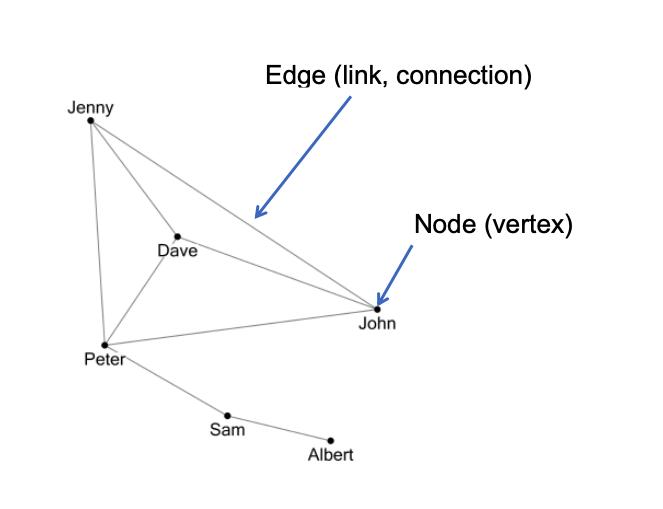
\includegraphics[width=0.9\linewidth,height=0.8\textheight]{./images/fb}
\ecenter
\end{frame}

\begin{frame}{Example: social network}
\protect\hypertarget{example-social-network-1}{}
Twitter: Directed network

\bcenter

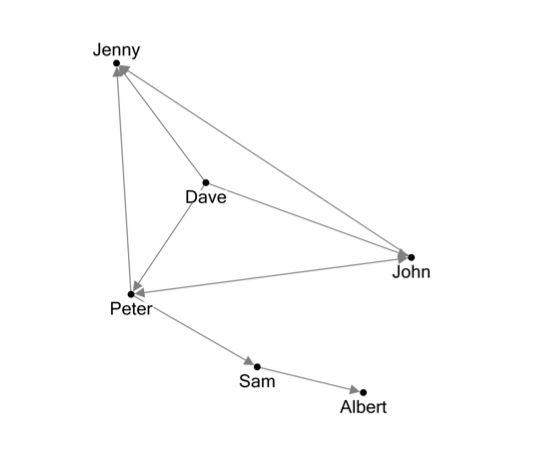
\includegraphics[width=0.9\linewidth,height=0.8\textheight]{./images/twitter}
\ecenter
\end{frame}

\begin{frame}[fragile]{Installing necessary packages}
\protect\hypertarget{installing-necessary-packages}{}
We will use 3 main packages for the network analsysis for creating and
manipulating graph objects

\begin{itemize}
\tightlist
\item
  igraph
\item
  network
\end{itemize}

For changing the class of objects from network to igraph and vice versa

\begin{itemize}
\tightlist
\item
  intergraph
\end{itemize}

\begin{Shaded}
\begin{Highlighting}[]
\FunctionTok{install.packages}\NormalTok{(}\StringTok{"igraph"}\NormalTok{)}
\FunctionTok{install.packages}\NormalTok{(}\StringTok{"network"}\NormalTok{)}
\FunctionTok{install.packages}\NormalTok{(}\StringTok{"intergraph"}\NormalTok{)}
\end{Highlighting}
\end{Shaded}
\end{frame}

\begin{frame}[fragile]{Tools for social network analysis}
\protect\hypertarget{tools-for-social-network-analysis}{}
\begin{itemize}
\tightlist
\item
  sna - A range of tools for social network analysis
\item
  statnet: metapackage statnet: installs everything you need
\item
  statnetweb: r shiny application for network analysis
\end{itemize}

\begin{Shaded}
\begin{Highlighting}[]
\FunctionTok{install.packages}\NormalTok{(}\StringTok{"sna"}\NormalTok{) }
\FunctionTok{install.packages}\NormalTok{(}\StringTok{"statnet"}\NormalTok{) }
\FunctionTok{install.packages}\NormalTok{(}\StringTok{"statnetWeb"}\NormalTok{)}
\end{Highlighting}
\end{Shaded}
\end{frame}

\begin{frame}{Types of data stored in the network data object}
\protect\hypertarget{types-of-data-stored-in-the-network-data-object}{}
\bcenter

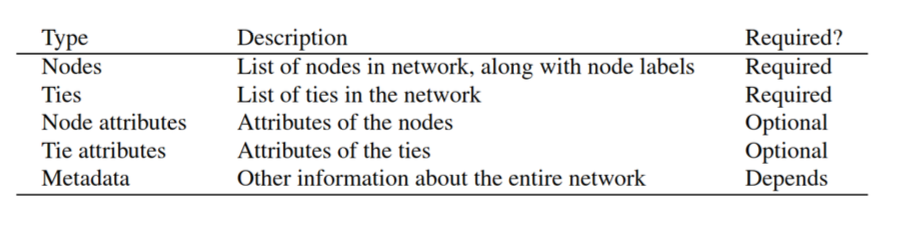
\includegraphics[width=0.9\linewidth,height=0.8\textheight]{./images/network_data_1}
\ecenter
\end{frame}

\begin{frame}{Input data}
\protect\hypertarget{input-data}{}
There are two main types of data structures that are used for network
analysis.

\begin{itemize}
\tightlist
\item
  Adjacency matrix (sociomatrix)
\item
  Edge list
\end{itemize}
\end{frame}

\begin{frame}[fragile]{Adjacency matrix}
\protect\hypertarget{adjacency-matrix}{}
An adjacency matrix is a square matrix where a 1 indicates a tie between
two nodes, and a 0 indicates no tie.

The convention is that rows indicate the starting node, and columns
indicate the receiving node

\begin{Shaded}
\begin{Highlighting}[]
\NormalTok{mat }\OtherTok{\textless{}{-}} \FunctionTok{rbind}\NormalTok{(}\FunctionTok{c}\NormalTok{(}\DecValTok{0}\NormalTok{,}\DecValTok{1}\NormalTok{,}\DecValTok{1}\NormalTok{,}\DecValTok{0}\NormalTok{,}\DecValTok{0}\NormalTok{),}\FunctionTok{c}\NormalTok{(}\DecValTok{0}\NormalTok{,}\DecValTok{0}\NormalTok{,}\DecValTok{1}\NormalTok{,}\DecValTok{1}\NormalTok{,}\DecValTok{0}\NormalTok{),}\FunctionTok{c}\NormalTok{(}\DecValTok{0}\NormalTok{,}\DecValTok{1}\NormalTok{,}\DecValTok{0}\NormalTok{,}\DecValTok{0}\NormalTok{,}\DecValTok{0}\NormalTok{),}
              \FunctionTok{c}\NormalTok{(}\DecValTok{0}\NormalTok{,}\DecValTok{0}\NormalTok{,}\DecValTok{0}\NormalTok{,}\DecValTok{0}\NormalTok{,}\DecValTok{0}\NormalTok{),}\FunctionTok{c}\NormalTok{(}\DecValTok{0}\NormalTok{,}\DecValTok{0}\NormalTok{,}\DecValTok{1}\NormalTok{,}\DecValTok{0}\NormalTok{,}\DecValTok{0}\NormalTok{))}
\FunctionTok{rownames}\NormalTok{(mat) }\OtherTok{\textless{}{-}} \FunctionTok{c}\NormalTok{(}\StringTok{"A"}\NormalTok{,}\StringTok{"B"}\NormalTok{,}\StringTok{"C"}\NormalTok{,}\StringTok{"D"}\NormalTok{,}\StringTok{"E"}\NormalTok{)}
\FunctionTok{colnames}\NormalTok{(mat) }\OtherTok{\textless{}{-}} \FunctionTok{c}\NormalTok{(}\StringTok{"A"}\NormalTok{,}\StringTok{"B"}\NormalTok{,}\StringTok{"C"}\NormalTok{,}\StringTok{"D"}\NormalTok{,}\StringTok{"E"}\NormalTok{)}
\NormalTok{mat}
\end{Highlighting}
\end{Shaded}

\begin{verbatim}
##   A B C D E
## A 0 1 1 0 0
## B 0 0 1 1 0
## C 0 1 0 0 0
## D 0 0 0 0 0
## E 0 0 1 0 0
\end{verbatim}
\end{frame}

\begin{frame}[fragile]{Adjacency matrix}
\protect\hypertarget{adjacency-matrix-1}{}
\tiny

\begin{Shaded}
\begin{Highlighting}[]
\NormalTok{net}\OtherTok{\textless{}{-}}\FunctionTok{network}\NormalTok{(mat, }\AttributeTok{matrix.type=}\StringTok{"adjacency"}\NormalTok{)}
\FunctionTok{summary}\NormalTok{(net)}
\end{Highlighting}
\end{Shaded}

\begin{verbatim}
## Network attributes:
##   vertices = 5
##   directed = TRUE
##   hyper = FALSE
##   loops = FALSE
##   multiple = FALSE
##   bipartite = FALSE
##  total edges = 6 
##    missing edges = 0 
##    non-missing edges = 6 
##  density = 0.3 
## 
## Vertex attributes:
##   vertex.names:
##    character valued attribute
##    5 valid vertex names
## 
## No edge attributes
## 
## Network adjacency matrix:
##   A B C D E
## A 0 1 1 0 0
## B 0 0 1 1 0
## C 0 1 0 0 0
## D 0 0 0 0 0
## E 0 0 1 0 0
\end{verbatim}
\end{frame}

\begin{frame}[fragile]{Plotting}
\protect\hypertarget{plotting}{}
\begin{Shaded}
\begin{Highlighting}[]
\FunctionTok{plot}\NormalTok{(net, }\AttributeTok{main=}\StringTok{"Network example"}\NormalTok{, }\AttributeTok{displaylabels=}\NormalTok{T)}
\end{Highlighting}
\end{Shaded}

\begin{center}\includegraphics{network_analysis_files/figure-beamer/unnamed-chunk-8-1} \end{center}
\end{frame}

\begin{frame}[fragile]{Plotting}
\protect\hypertarget{plotting-1}{}
Add the vertex labels with \textbf{\emph{label=network.vertex.names()}}

\begin{Shaded}
\begin{Highlighting}[]
\FunctionTok{plot}\NormalTok{(net, }\AttributeTok{main=}\StringTok{"Network example"}\NormalTok{, }\AttributeTok{label=}\FunctionTok{network.vertex.names}\NormalTok{(net))}
\end{Highlighting}
\end{Shaded}

\begin{center}\includegraphics{network_analysis_files/figure-beamer/unnamed-chunk-9-1} \end{center}
\end{frame}

\begin{frame}[fragile]{Plotting}
\protect\hypertarget{plotting-2}{}
You can increase the vertex size by the parameter
\textbf{\emph{vertex.cex}}

\begin{Shaded}
\begin{Highlighting}[]
\FunctionTok{plot}\NormalTok{(net, }\AttributeTok{main=}\StringTok{"Network example"}\NormalTok{, }\AttributeTok{label=}\FunctionTok{network.vertex.names}\NormalTok{(net), }\AttributeTok{vertex.cex=}\FloatTok{2.5}\NormalTok{)}
\end{Highlighting}
\end{Shaded}

\begin{center}\includegraphics{network_analysis_files/figure-beamer/unnamed-chunk-10-1} \end{center}
\end{frame}

\begin{frame}[fragile]{Plotting}
\protect\hypertarget{plotting-3}{}
Increase the labels size with \textbf{\emph{label.cex}}

\begin{Shaded}
\begin{Highlighting}[]
\FunctionTok{plot}\NormalTok{(net, }\AttributeTok{main=}\StringTok{"Network example"}\NormalTok{, }
     \AttributeTok{label=}\FunctionTok{network.vertex.names}\NormalTok{(net), }\AttributeTok{vertex.cex=}\FloatTok{2.5}\NormalTok{, }\AttributeTok{label.cex=}\FloatTok{1.5}\NormalTok{)}
\end{Highlighting}
\end{Shaded}

\begin{center}\includegraphics{network_analysis_files/figure-beamer/unnamed-chunk-11-1} \end{center}
\end{frame}

\begin{frame}[fragile]{Plotting}
\protect\hypertarget{plotting-4}{}
Increase the edge size with \textbf{\emph{edge.lwd}} \tiny

\begin{Shaded}
\begin{Highlighting}[]
\FunctionTok{plot}\NormalTok{(net, }\AttributeTok{main=}\StringTok{"Network example"}\NormalTok{, }
     \AttributeTok{label=}\FunctionTok{network.vertex.names}\NormalTok{(net), }\AttributeTok{vertex.cex=}\FloatTok{2.5}\NormalTok{, }\AttributeTok{label.cex=}\FloatTok{1.5}\NormalTok{, }\AttributeTok{edge.lwd=}\DecValTok{10}\NormalTok{)}
\end{Highlighting}
\end{Shaded}

\begin{center}\includegraphics[height=0.8\textheight]{network_analysis_files/figure-beamer/unnamed-chunk-12-1} \end{center}
\end{frame}

\begin{frame}[fragile]{Edge list}
\protect\hypertarget{edge-list}{}
Edge list is a form of representing the network data, where each node is
a tie/edge, with two columns specifying the FROM and TO nodes

Edge list for the previous example

\begin{Shaded}
\begin{Highlighting}[]
\NormalTok{mat1}\OtherTok{\textless{}{-}}\FunctionTok{cbind}\NormalTok{(}\AttributeTok{FROM=}\FunctionTok{c}\NormalTok{(}\StringTok{"A"}\NormalTok{, }\StringTok{"A"}\NormalTok{, }\StringTok{"B"}\NormalTok{, }\StringTok{"B"}\NormalTok{, }\StringTok{"C"}\NormalTok{, }\StringTok{"E"}\NormalTok{),}
            \AttributeTok{TO=}\FunctionTok{c}\NormalTok{(}\StringTok{"B"}\NormalTok{, }\StringTok{"C"}\NormalTok{, }\StringTok{"C"}\NormalTok{, }\StringTok{"D"}\NormalTok{, }\StringTok{"B"}\NormalTok{, }\StringTok{"C"}\NormalTok{))}
\NormalTok{mat1}
\end{Highlighting}
\end{Shaded}

\begin{verbatim}
##      FROM TO 
## [1,] "A"  "B"
## [2,] "A"  "C"
## [3,] "B"  "C"
## [4,] "B"  "D"
## [5,] "C"  "B"
## [6,] "E"  "C"
\end{verbatim}
\end{frame}

\begin{frame}[fragile]{Edge list}
\protect\hypertarget{edge-list-1}{}
Specify \textbf{\emph{matrix.type=``edgelist''}}

\begin{Shaded}
\begin{Highlighting}[]
\NormalTok{net1}\OtherTok{\textless{}{-}}\FunctionTok{network}\NormalTok{(mat1, }\AttributeTok{matrix.type=}\StringTok{"edgelist"}\NormalTok{)}
\end{Highlighting}
\end{Shaded}

\tiny

\begin{Shaded}
\begin{Highlighting}[]
\FunctionTok{plot}\NormalTok{(net1, }\AttributeTok{main=}\StringTok{"Network example"}\NormalTok{, }
     \AttributeTok{label=}\FunctionTok{network.vertex.names}\NormalTok{(net), }\AttributeTok{vertex.cex=}\FloatTok{2.5}\NormalTok{, }\AttributeTok{label.cex=}\FloatTok{1.5}\NormalTok{, }\AttributeTok{edge.lwd=}\DecValTok{10}\NormalTok{)}
\end{Highlighting}
\end{Shaded}

\begin{center}\includegraphics[height=0.6\textheight]{network_analysis_files/figure-beamer/unnamed-chunk-15-1} \end{center}
\end{frame}

\begin{frame}[fragile]{With igraph}
\protect\hypertarget{with-igraph}{}
We can also get the edge list from the network object

\begin{Shaded}
\begin{Highlighting}[]
\NormalTok{net\_ed}\OtherTok{\textless{}{-}}\FunctionTok{as.matrix}\NormalTok{(net,}\AttributeTok{matrix.type =} \StringTok{"edgelist"}\NormalTok{)}
\NormalTok{net\_ed}
\end{Highlighting}
\end{Shaded}

\begin{verbatim}
##      [,1] [,2]
## [1,]    1    2
## [2,]    3    2
## [3,]    1    3
## [4,]    2    3
## [5,]    5    3
## [6,]    2    4
## attr(,"n")
## [1] 5
## attr(,"vnames")
## [1] "A" "B" "C" "D" "E"
\end{verbatim}
\end{frame}

\begin{frame}[fragile]{Using igraph}
\protect\hypertarget{using-igraph}{}
\begin{Shaded}
\begin{Highlighting}[]
\NormalTok{net3}\OtherTok{\textless{}{-}}\NormalTok{igraph}\SpecialCharTok{::}\FunctionTok{graph\_from\_edgelist}\NormalTok{(net\_ed)}
\FunctionTok{plot}\NormalTok{(net3)}
\end{Highlighting}
\end{Shaded}

\begin{center}\includegraphics[height=0.8\textheight]{network_analysis_files/figure-beamer/unnamed-chunk-17-1} \end{center}
\end{frame}

\begin{frame}[fragile]{With igraph}
\protect\hypertarget{with-igraph-1}{}
Create graph using adjacency matrix with igraph

\begin{Shaded}
\begin{Highlighting}[]
\NormalTok{net4}\OtherTok{\textless{}{-}}\FunctionTok{graph\_from\_adjacency\_matrix}\NormalTok{(mat)}
\FunctionTok{plot}\NormalTok{(net4)}
\end{Highlighting}
\end{Shaded}

\begin{center}\includegraphics[height=0.7\textheight]{network_analysis_files/figure-beamer/unnamed-chunk-18-1} \end{center}
\end{frame}

\begin{frame}[fragile]{Vizualizing with gplot}
\protect\hypertarget{vizualizing-with-gplot}{}
\begin{Shaded}
\begin{Highlighting}[]
\NormalTok{sna}\SpecialCharTok{::}\FunctionTok{gplot}\NormalTok{(net1, }\AttributeTok{displaylabels =}\NormalTok{ T)}
\end{Highlighting}
\end{Shaded}

\begin{center}\includegraphics[height=0.8\textheight]{network_analysis_files/figure-beamer/unnamed-chunk-19-1} \end{center}
\end{frame}

\begin{frame}[fragile]{Converting from igraph to network and vice versa}
\protect\hypertarget{converting-from-igraph-to-network-and-vice-versa}{}
\begin{Shaded}
\begin{Highlighting}[]
\NormalTok{net\_i}\OtherTok{\textless{}{-}}\NormalTok{intergraph}\SpecialCharTok{::}\FunctionTok{asIgraph}\NormalTok{(net1)}
\FunctionTok{class}\NormalTok{(net\_i)}
\end{Highlighting}
\end{Shaded}

\begin{verbatim}
## [1] "igraph"
\end{verbatim}

vice versa

\begin{Shaded}
\begin{Highlighting}[]
\NormalTok{net\_n}\OtherTok{\textless{}{-}}\NormalTok{intergraph}\SpecialCharTok{::}\FunctionTok{asNetwork}\NormalTok{(net\_i)}
\FunctionTok{class}\NormalTok{(net\_n)}
\end{Highlighting}
\end{Shaded}

\begin{verbatim}
## [1] "network"
\end{verbatim}
\end{frame}

\begin{frame}[fragile]{Adding vertex attributes with network package}
\protect\hypertarget{adding-vertex-attributes-with-network-package}{}
\tiny

\begin{Shaded}
\begin{Highlighting}[]
\CommentTok{\# object from network package}
\NormalTok{network}\SpecialCharTok{::}\FunctionTok{set.vertex.attribute}\NormalTok{(net1, }\StringTok{"gender"}\NormalTok{, }\FunctionTok{c}\NormalTok{(}\StringTok{"F"}\NormalTok{, }\StringTok{"F"}\NormalTok{, }\StringTok{"M"}\NormalTok{, }\StringTok{"F"}\NormalTok{, }\StringTok{"M"}\NormalTok{))}
\FunctionTok{summary}\NormalTok{(net1)}
\end{Highlighting}
\end{Shaded}

\begin{verbatim}
## Network attributes:
##   vertices = 5
##   directed = TRUE
##   hyper = FALSE
##   loops = FALSE
##   multiple = FALSE
##   bipartite = FALSE
##  total edges = 6 
##    missing edges = 0 
##    non-missing edges = 6 
##  density = 0.3 
## 
## Vertex attributes:
## 
##  gender:
##    character valued attribute
##    attribute summary:
## F M 
## 3 2 
##   vertex.names:
##    character valued attribute
##    5 valid vertex names
## 
## No edge attributes
## 
## Network adjacency matrix:
##   A B C D E
## A 0 1 1 0 0
## B 0 0 1 1 0
## C 0 1 0 0 0
## D 0 0 0 0 0
## E 0 0 1 0 0
\end{verbatim}
\end{frame}

\begin{frame}[fragile]{Adding vertex attributes with network package}
\protect\hypertarget{adding-vertex-attributes-with-network-package-1}{}
\begin{Shaded}
\begin{Highlighting}[]
\NormalTok{network}\SpecialCharTok{::}\FunctionTok{get.vertex.attribute}\NormalTok{(net1, }\StringTok{"gender"}\NormalTok{)}
\end{Highlighting}
\end{Shaded}

\begin{verbatim}
## [1] "F" "F" "M" "F" "M"
\end{verbatim}

\begin{Shaded}
\begin{Highlighting}[]
\CommentTok{\# The same}
\NormalTok{net1 }\SpecialCharTok{\%v\%} \StringTok{"gender"}
\end{Highlighting}
\end{Shaded}

\begin{verbatim}
## [1] "F" "F" "M" "F" "M"
\end{verbatim}
\end{frame}

\begin{frame}[fragile]{Vertex attributes}
\protect\hypertarget{vertex-attributes}{}
Plot by coloring with network attribute

\begin{Shaded}
\begin{Highlighting}[]
\FunctionTok{plot}\NormalTok{(net1,}\AttributeTok{label=}\FunctionTok{network.vertex.names}\NormalTok{(net1), }
     \AttributeTok{vertex.cex=}\FloatTok{2.5}\NormalTok{, }\AttributeTok{label.cex=}\FloatTok{1.5}\NormalTok{,}
     \AttributeTok{main=}\StringTok{"Sample graph with node attributes"}\NormalTok{,}
     \AttributeTok{vertex.col=}\StringTok{"gender"}\NormalTok{)}
\end{Highlighting}
\end{Shaded}

\includegraphics[height=0.7\textheight]{network_analysis_files/figure-beamer/unnamed-chunk-24-1}
\end{frame}

\begin{frame}[fragile]{Adding edge attribute}
\protect\hypertarget{adding-edge-attribute}{}
\begin{Shaded}
\begin{Highlighting}[]
\NormalTok{network}\SpecialCharTok{::}\FunctionTok{set.edge.attribute}\NormalTok{(net1, }\StringTok{"edge.size"}\NormalTok{, }\FunctionTok{c}\NormalTok{(}\DecValTok{3}\NormalTok{,}\DecValTok{0}\NormalTok{,}\DecValTok{5}\NormalTok{,}\DecValTok{2}\NormalTok{,}\DecValTok{6}\NormalTok{))}
\CommentTok{\# Check if added}
\NormalTok{network}\SpecialCharTok{::}\FunctionTok{get.edge.attribute}\NormalTok{(net1, }\StringTok{"edge.size"}\NormalTok{)}
\end{Highlighting}
\end{Shaded}

\begin{verbatim}
## [1] 3 0 5 2 6 3
\end{verbatim}

\begin{Shaded}
\begin{Highlighting}[]
\CommentTok{\# the same}
\NormalTok{net1 }\SpecialCharTok{\%e\%} \StringTok{"edge.size"}
\end{Highlighting}
\end{Shaded}

\begin{verbatim}
## [1] 3 0 5 2 6 3
\end{verbatim}
\end{frame}

\begin{frame}[fragile]{Looking what is inside: List node and edge
attributes}
\protect\hypertarget{looking-what-is-inside-list-node-and-edge-attributes}{}
\begin{Shaded}
\begin{Highlighting}[]
\NormalTok{network}\SpecialCharTok{::}\FunctionTok{list.vertex.attributes}\NormalTok{(net1)}
\end{Highlighting}
\end{Shaded}

\begin{verbatim}
## [1] "gender"       "na"           "vertex.names"
\end{verbatim}

\begin{Shaded}
\begin{Highlighting}[]
\NormalTok{network}\SpecialCharTok{::}\FunctionTok{list.edge.attributes}\NormalTok{(net1)}
\end{Highlighting}
\end{Shaded}

\begin{verbatim}
## [1] "edge.size" "na"
\end{verbatim}
\end{frame}

\begin{frame}[fragile]{Plotting Edge Attributes}
\protect\hypertarget{plotting-edge-attributes}{}
Edge attribute as an edge label,
\textbf{\emph{edge.label=``edge.size''}}

\begin{Shaded}
\begin{Highlighting}[]
\FunctionTok{plot}\NormalTok{(net1,}\AttributeTok{label=}\FunctionTok{network.vertex.names}\NormalTok{(net1), }
     \AttributeTok{vertex.cex=}\FloatTok{2.5}\NormalTok{, }\AttributeTok{label.cex=}\FloatTok{1.5}\NormalTok{,}
     \AttributeTok{main=}\StringTok{"Sample graph with node attributes"}\NormalTok{,}
     \AttributeTok{vertex.col=}\StringTok{"gender"}\NormalTok{, }\AttributeTok{edge.label=}\StringTok{"edge.size"}\NormalTok{)}
\end{Highlighting}
\end{Shaded}

\includegraphics[height=0.6\textheight]{network_analysis_files/figure-beamer/page_28-1}
\end{frame}

\begin{frame}[fragile]{Plotting Edge attribute}
\protect\hypertarget{plotting-edge-attribute}{}
Edge attribute is used to set edge size, with
\textbf{\emph{edge.lwd=``edge.size''}}

\begin{Shaded}
\begin{Highlighting}[]
\FunctionTok{plot}\NormalTok{(net1,}\AttributeTok{label=}\FunctionTok{network.vertex.names}\NormalTok{(net1), }
     \AttributeTok{vertex.cex=}\FloatTok{2.5}\NormalTok{, }\AttributeTok{label.cex=}\FloatTok{1.5}\NormalTok{, }
     \AttributeTok{main=}\StringTok{"Sample graph with node attributes"}\NormalTok{,}
     \AttributeTok{vertex.col=}\StringTok{"gender"}\NormalTok{)}
\end{Highlighting}
\end{Shaded}

\includegraphics[height=0.6\textheight]{network_analysis_files/figure-beamer/page_29-1}
\end{frame}

\begin{frame}{Graph layout}
\protect\hypertarget{graph-layout}{}
\begin{itemize}
\tightlist
\item
  The graph layout (the nodes coordinates) are drawn randomly
\item
  So every time you make the same graph, you are going to get different
  picture Solutions (if it is a problem at all)
\item
  use set.seed() to get the same graph
\item
  Save the coordinates
\item
  Use predefined layouts
\end{itemize}
\end{frame}

\begin{frame}[fragile]{Graph layout}
\protect\hypertarget{graph-layout-1}{}
use set.seed() when running the plot command

\begin{Shaded}
\begin{Highlighting}[]
\FunctionTok{set.seed}\NormalTok{(}\DecValTok{1}\NormalTok{)}
\FunctionTok{plot}\NormalTok{(net1,}\AttributeTok{label=}\FunctionTok{network.vertex.names}\NormalTok{(net1))}
\end{Highlighting}
\end{Shaded}

\includegraphics{network_analysis_files/figure-beamer/unnamed-chunk-27-1.pdf}
\end{frame}

\begin{frame}[fragile]{Graph layout}
\protect\hypertarget{graph-layout-2}{}
Make the coordinates matrix

\begin{Shaded}
\begin{Highlighting}[]
\FunctionTok{set.seed}\NormalTok{(}\DecValTok{1}\NormalTok{)}
\NormalTok{my\_coord}\OtherTok{\textless{}{-}}\FunctionTok{plot}\NormalTok{(net1,}\AttributeTok{displaylabels=}\NormalTok{T)}
\end{Highlighting}
\end{Shaded}

\includegraphics{network_analysis_files/figure-beamer/unnamed-chunk-28-1.pdf}

\begin{Shaded}
\begin{Highlighting}[]
\NormalTok{my\_coord}
\end{Highlighting}
\end{Shaded}

\begin{verbatim}
##              cx        cy
## [1,] -2.8302013 -7.143824
## [2,] -1.2741967 -7.175849
## [3,] -2.0958007 -5.787260
## [4,]  0.2592268 -7.492759
## [5,] -1.6911682 -4.286334
\end{verbatim}
\end{frame}

\begin{frame}[fragile]{Graph layout}
\protect\hypertarget{graph-layout-3}{}
Use argument coord

\begin{Shaded}
\begin{Highlighting}[]
\FunctionTok{plot}\NormalTok{(net1,}\AttributeTok{label=}\FunctionTok{network.vertex.names}\NormalTok{(net1), }\AttributeTok{coord=}\NormalTok{my\_coord)}
\end{Highlighting}
\end{Shaded}

\includegraphics{network_analysis_files/figure-beamer/unnamed-chunk-29-1.pdf}
\end{frame}

\begin{frame}{Graph layout}
\protect\hypertarget{graph-layout-4}{}
You can use also predefined layouts, such as

\begin{itemize}
\tightlist
\item
  Circle
\item
  Fruchterman Reingold
\item
  Kamada-Kawai
\item
  Random
\end{itemize}
\end{frame}

\begin{frame}{Graph layout}
\protect\hypertarget{graph-layout-5}{}
\bcenter

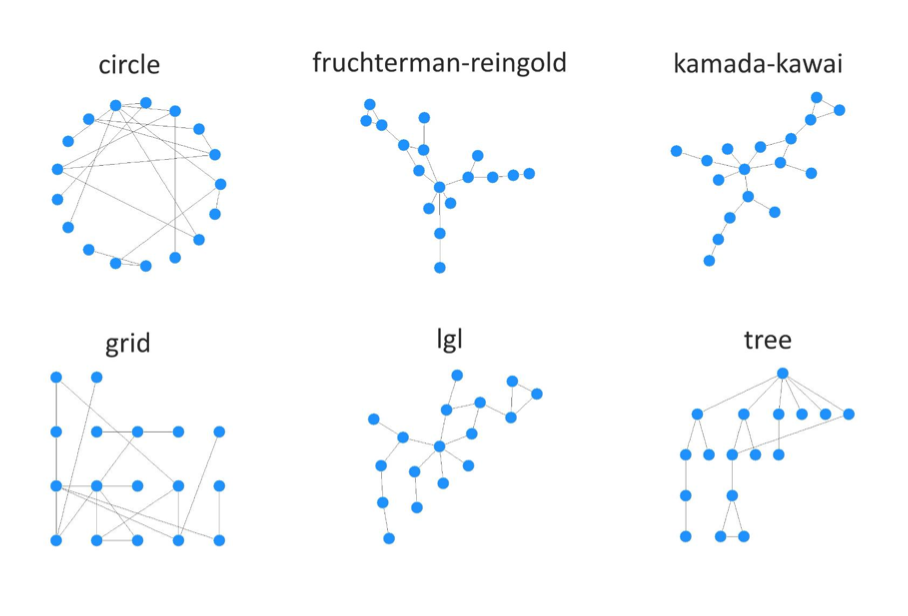
\includegraphics[width=0.9\linewidth,height=0.8\textheight]{./images/layout_1}
\ecenter
\end{frame}

\begin{frame}[fragile]{Graph layout: network package}
\protect\hypertarget{graph-layout-network-package}{}
Set argument \textbf{\emph{mode=``circle''}}

\begin{Shaded}
\begin{Highlighting}[]
\FunctionTok{plot}\NormalTok{(net1,}\AttributeTok{label=}\FunctionTok{network.vertex.names}\NormalTok{(net1), }
     \AttributeTok{mode=}\StringTok{"circle"}\NormalTok{, }\AttributeTok{main=}\StringTok{"Circle Layout"}\NormalTok{)}
\end{Highlighting}
\end{Shaded}

\includegraphics[height=0.7\textheight]{network_analysis_files/figure-beamer/unnamed-chunk-31-1}
\end{frame}

\begin{frame}[fragile]{Graph layout}
\protect\hypertarget{graph-layout-6}{}
\begin{Shaded}
\begin{Highlighting}[]
\FunctionTok{plot}\NormalTok{(net1,}\AttributeTok{label=}\FunctionTok{network.vertex.names}\NormalTok{(net1), }
     \AttributeTok{mode=}\StringTok{"fruchtermanreingold"}\NormalTok{, }
     \AttributeTok{main=}\StringTok{"Fruchterman {-} Reingold: The default layout"}\NormalTok{)}
\end{Highlighting}
\end{Shaded}

\includegraphics[height=0.7\textheight]{network_analysis_files/figure-beamer/unnamed-chunk-32-1}
\end{frame}

\begin{frame}[fragile]{Graph layout}
\protect\hypertarget{graph-layout-7}{}
\begin{Shaded}
\begin{Highlighting}[]
\FunctionTok{plot}\NormalTok{(net1,}\AttributeTok{label=}\FunctionTok{network.vertex.names}\NormalTok{(net1), }
     \AttributeTok{mode=}\StringTok{"kamadakawai"}\NormalTok{, }\AttributeTok{main=}\StringTok{"Kamada{-}kawai"}\NormalTok{)}
\end{Highlighting}
\end{Shaded}

\includegraphics[height=0.7\textheight]{network_analysis_files/figure-beamer/unnamed-chunk-33-1}
\end{frame}

\begin{frame}[fragile]{Graph layout: igraph}
\protect\hypertarget{graph-layout-igraph}{}
With igraph package

\begin{Shaded}
\begin{Highlighting}[]
\NormalTok{net5}\OtherTok{\textless{}{-}}\FunctionTok{asIgraph}\NormalTok{(net1)}
\NormalTok{coords}\OtherTok{\textless{}{-}}\FunctionTok{layout\_in\_circle}\NormalTok{(net5)}
\NormalTok{coords}
\end{Highlighting}
\end{Shaded}

\begin{verbatim}
##           [,1]       [,2]
## [1,]  1.000000  0.0000000
## [2,]  0.309017  0.9510565
## [3,] -0.809017  0.5877853
## [4,] -0.809017 -0.5877853
## [5,]  0.309017 -0.9510565
\end{verbatim}

Note: Coordinates are generated randomly, so if you don't specify
set.seed() you are going to have different results every time
\end{frame}

\begin{frame}[fragile]{Graph layout}
\protect\hypertarget{graph-layout-8}{}
\begin{Shaded}
\begin{Highlighting}[]
\FunctionTok{plot}\NormalTok{(net5, }\AttributeTok{layout=}\NormalTok{coords, }\AttributeTok{main=}\StringTok{"Circle Layout"}\NormalTok{)}
\end{Highlighting}
\end{Shaded}

\includegraphics{network_analysis_files/figure-beamer/unnamed-chunk-35-1.pdf}
\end{frame}

\begin{frame}[fragile]{Graph layout}
\protect\hypertarget{graph-layout-9}{}
\begin{Shaded}
\begin{Highlighting}[]
\FunctionTok{plot}\NormalTok{(net5, }\AttributeTok{layout=}\FunctionTok{layout\_with\_fr}\NormalTok{(net5), }\AttributeTok{main=}\StringTok{"Fruchterman {-} Reingold"}\NormalTok{)}
\end{Highlighting}
\end{Shaded}

\includegraphics{network_analysis_files/figure-beamer/unnamed-chunk-36-1.pdf}
\end{frame}

\begin{frame}[fragile]{Graph layout}
\protect\hypertarget{graph-layout-10}{}
\begin{Shaded}
\begin{Highlighting}[]
\FunctionTok{plot}\NormalTok{(net5, }\AttributeTok{layout=}\FunctionTok{layout\_on\_grid}\NormalTok{(net5), }\AttributeTok{main=}\StringTok{"Grid layout"}\NormalTok{)}
\end{Highlighting}
\end{Shaded}

\includegraphics{network_analysis_files/figure-beamer/unnamed-chunk-37-1.pdf}
\end{frame}

\begin{frame}[fragile]{Graph layout}
\protect\hypertarget{graph-layout-11}{}
\begin{Shaded}
\begin{Highlighting}[]
\FunctionTok{plot}\NormalTok{(net5, }\AttributeTok{layout=}\FunctionTok{layout\_nicely}\NormalTok{(net5), }\AttributeTok{main=}\StringTok{"Nice layout"}\NormalTok{)}
\end{Highlighting}
\end{Shaded}

\includegraphics{network_analysis_files/figure-beamer/unnamed-chunk-38-1.pdf}
\end{frame}

\begin{frame}[fragile]{Graphing with coordinates}
\protect\hypertarget{graphing-with-coordinates}{}
Altering the coordinates

\begin{Shaded}
\begin{Highlighting}[]
\FunctionTok{set.seed}\NormalTok{(}\DecValTok{1}\NormalTok{)}
\NormalTok{coord1}\OtherTok{\textless{}{-}}\FunctionTok{plot}\NormalTok{(net1,}\AttributeTok{displaylabels=}\NormalTok{T, }\AttributeTok{mode=}\StringTok{"circle"}\NormalTok{, }\AttributeTok{main=}\StringTok{"Circle Layout"}\NormalTok{, }\AttributeTok{suppress.axes=}\NormalTok{F)}
\end{Highlighting}
\end{Shaded}

\includegraphics[height=0.7\textheight]{network_analysis_files/figure-beamer/unnamed-chunk-39-1}
\end{frame}

\begin{frame}[fragile]{Altering the coordinates}
\protect\hypertarget{altering-the-coordinates}{}
Lets say you want to bring Node C to the center

\begin{Shaded}
\begin{Highlighting}[]
\CommentTok{\#C is the third node, set coordinates to zero}
\NormalTok{coord1[}\DecValTok{3}\NormalTok{,]}\OtherTok{\textless{}{-}}\DecValTok{0}
\FunctionTok{plot}\NormalTok{(net1,}\AttributeTok{displaylabels=}\NormalTok{T, }\AttributeTok{mode=}\StringTok{"circle"}\NormalTok{, }\AttributeTok{main=}\StringTok{"Circle Layout"}\NormalTok{, }\AttributeTok{coord=}\NormalTok{coord1)}
\end{Highlighting}
\end{Shaded}

\includegraphics[height=0.7\textheight]{network_analysis_files/figure-beamer/unnamed-chunk-40-1}
\end{frame}

\begin{frame}[fragile]{Sub setting the graph: by vertex attribute}
\protect\hypertarget{sub-setting-the-graph-by-vertex-attribute}{}
\begin{Shaded}
\begin{Highlighting}[]
\CommentTok{\# library network}
\NormalTok{net1 }\SpecialCharTok{\%v\%} \StringTok{"gender"}
\end{Highlighting}
\end{Shaded}

\begin{verbatim}
## [1] "F" "F" "M" "F" "M"
\end{verbatim}

\begin{Shaded}
\begin{Highlighting}[]
\NormalTok{net\_f}\OtherTok{\textless{}{-}}\FunctionTok{get.inducedSubgraph}\NormalTok{(net1, }\AttributeTok{v=}\FunctionTok{which}\NormalTok{(net1 }\SpecialCharTok{\%v\%} \StringTok{"gender"} \SpecialCharTok{==} \StringTok{"F"}\NormalTok{))}
\FunctionTok{plot}\NormalTok{(net\_f, }\AttributeTok{label=}\FunctionTok{network.vertex.names}\NormalTok{(net\_f))}
\end{Highlighting}
\end{Shaded}

\includegraphics[height=0.6\textheight]{network_analysis_files/figure-beamer/unnamed-chunk-41-1}
\end{frame}

\begin{frame}[fragile]{Sub setting the graph: by edge attribute}
\protect\hypertarget{sub-setting-the-graph-by-edge-attribute}{}
\begin{Shaded}
\begin{Highlighting}[]
\NormalTok{net1 }\SpecialCharTok{\%e\%} \StringTok{"edge.size"}
\end{Highlighting}
\end{Shaded}

\begin{verbatim}
## [1] 3 0 5 2 6 3
\end{verbatim}

\begin{Shaded}
\begin{Highlighting}[]
\CommentTok{\# get the edges for which the edge.size is \textgreater{}= 3}
\NormalTok{net\_e}\OtherTok{\textless{}{-}}\FunctionTok{get.inducedSubgraph}\NormalTok{(net1, }\AttributeTok{eid=}\FunctionTok{which}\NormalTok{(net1 }\SpecialCharTok{\%e\%} \StringTok{"edge.size"} \SpecialCharTok{\textgreater{}=}\DecValTok{3}\NormalTok{))}
\FunctionTok{plot}\NormalTok{(net\_e, }\AttributeTok{label=}\FunctionTok{network.vertex.names}\NormalTok{(net\_e))}
\end{Highlighting}
\end{Shaded}

\includegraphics[height=0.7\textheight]{network_analysis_files/figure-beamer/unnamed-chunk-42-1}
\end{frame}

\begin{frame}[fragile]{Accessing network information with igraph}
\protect\hypertarget{accessing-network-information-with-igraph}{}
For vertex attributes

\begin{Shaded}
\begin{Highlighting}[]
\FunctionTok{class}\NormalTok{(net4)}
\end{Highlighting}
\end{Shaded}

\begin{verbatim}
## [1] "igraph"
\end{verbatim}

\begin{Shaded}
\begin{Highlighting}[]
\NormalTok{net4}\OtherTok{\textless{}{-}}\FunctionTok{set\_vertex\_attr}\NormalTok{(net4,}\StringTok{"gender"}\NormalTok{, }\AttributeTok{value=}\FunctionTok{c}\NormalTok{(}\StringTok{"F"}\NormalTok{, }\StringTok{"F"}\NormalTok{, }\StringTok{"M"}\NormalTok{,}
\StringTok{"F"}\NormalTok{, }\StringTok{"M"}\NormalTok{))}
\CommentTok{\# Accesing the vertex attribute}
\FunctionTok{V}\NormalTok{(net4)}\SpecialCharTok{$}\NormalTok{gender}
\end{Highlighting}
\end{Shaded}

\begin{verbatim}
## [1] "F" "F" "M" "F" "M"
\end{verbatim}

\begin{Shaded}
\begin{Highlighting}[]
\FunctionTok{V}\NormalTok{(net4)}\SpecialCharTok{$}\NormalTok{name}
\end{Highlighting}
\end{Shaded}

\begin{verbatim}
## [1] "A" "B" "C" "D" "E"
\end{verbatim}
\end{frame}

\begin{frame}[fragile]{Altering vertex attributes with igraph}
\protect\hypertarget{altering-vertex-attributes-with-igraph}{}
Setting edge attributes

\begin{Shaded}
\begin{Highlighting}[]
\CommentTok{\# altering the values of attributes}
\CommentTok{\# change the first element of the gender attribute to M}
\FunctionTok{V}\NormalTok{(net4)}\SpecialCharTok{$}\NormalTok{gender[}\DecValTok{1}\NormalTok{]}\OtherTok{\textless{}{-}}\StringTok{"M"}
\FunctionTok{V}\NormalTok{(net4)}\SpecialCharTok{$}\NormalTok{gender}
\end{Highlighting}
\end{Shaded}

\begin{verbatim}
## [1] "M" "F" "M" "F" "M"
\end{verbatim}
\end{frame}

\begin{frame}{Marvel Network}
\protect\hypertarget{marvel-network}{}
\begin{block}{Marvel Network}
\protect\hypertarget{marvel-network-1}{}
\end{block}
\end{frame}

\begin{frame}{Marvel network}
\protect\hypertarget{marvel-network-2}{}
\bcenter


\includegraphics[width=0.9\linewidth,height=0.8\textheight]{./images/marvel_1}
\ecenter
\end{frame}

\begin{frame}[fragile]{Marvel network}
\protect\hypertarget{marvel-network-3}{}
Number of common characters in the movies row 1: Ant Man and Avengers
Age of Ultron have 2 common characters

\begin{Shaded}
\begin{Highlighting}[]
\NormalTok{marvel }\OtherTok{\textless{}{-}} \FunctionTok{read.csv}\NormalTok{(}\StringTok{"./data/marvel.csv"}\NormalTok{)}
\FunctionTok{head}\NormalTok{(marvel)}
\end{Highlighting}
\end{Shaded}

\begin{verbatim}
##        V1                    V2 V3
## 1 Ant_Man     Ave_Age_Of_Ultron  2
## 2 Ant_Man          CA_Civil_War  4
## 3 Ant_Man  CA_The_First_Avenger  2
## 4 Ant_Man CA_The_Winter_Soldier  2
## 5 Ant_Man              Iron_Man  1
## 6 Ant_Man            Iron_Man_2  1
\end{verbatim}
\end{frame}

\begin{frame}[fragile]{Marvel network}
\protect\hypertarget{marvel-network-4}{}
\begin{itemize}
\tightlist
\item
  We will create a network where movies are going to be the vertices and
  the edges are going to show if two movies have common characters.
\item
  First create a network/igraph object
\end{itemize}

\begin{Shaded}
\begin{Highlighting}[]
\NormalTok{m\_igraph }\OtherTok{\textless{}{-}}\NormalTok{ igraph}\SpecialCharTok{::}\FunctionTok{graph\_from\_edgelist}\NormalTok{(}\FunctionTok{as.matrix}\NormalTok{(marvel[,}\DecValTok{1}\SpecialCharTok{:}\DecValTok{2}\NormalTok{]), }\AttributeTok{directed =}\NormalTok{ F)}
\NormalTok{m\_igraph }\OtherTok{\textless{}{-}} \FunctionTok{set\_edge\_attr}\NormalTok{(m\_igraph, }\StringTok{"characters"}\NormalTok{, }\AttributeTok{value =}\NormalTok{ marvel[,}\DecValTok{3}\NormalTok{])}
\FunctionTok{class}\NormalTok{(m\_igraph)}
\end{Highlighting}
\end{Shaded}

\begin{verbatim}
## [1] "igraph"
\end{verbatim}
\end{frame}

\begin{frame}[fragile]{Marvel network}
\protect\hypertarget{marvel-network-5}{}
\begin{Shaded}
\begin{Highlighting}[]
\FunctionTok{plot}\NormalTok{(m\_igraph, }\AttributeTok{layout =} \FunctionTok{layout\_in\_circle}\NormalTok{(m\_igraph))}
\end{Highlighting}
\end{Shaded}

\includegraphics{network_analysis_files/figure-beamer/unnamed-chunk-48-1.pdf}
\end{frame}

\begin{frame}[fragile]{Marvel network}
\protect\hypertarget{marvel-network-6}{}
Convert to network object

\begin{Shaded}
\begin{Highlighting}[]
\NormalTok{m\_net }\OtherTok{\textless{}{-}}\NormalTok{ intergraph}\SpecialCharTok{::}\FunctionTok{asNetwork}\NormalTok{(m\_igraph)}
\FunctionTok{plot}\NormalTok{(m\_net)}
\end{Highlighting}
\end{Shaded}

\includegraphics{network_analysis_files/figure-beamer/unnamed-chunk-49-1.pdf}
\end{frame}

\begin{frame}[fragile]{Marvel network}
\protect\hypertarget{marvel-network-7}{}
\begin{Shaded}
\begin{Highlighting}[]
\FunctionTok{plot}\NormalTok{(m\_net, }\AttributeTok{mode=}\StringTok{"circle"}\NormalTok{, }\AttributeTok{displaylabels=}\NormalTok{T, }\AttributeTok{label.pos=}\DecValTok{6}\NormalTok{)}
\end{Highlighting}
\end{Shaded}

\includegraphics{network_analysis_files/figure-beamer/unnamed-chunk-50-1.pdf}
\end{frame}

\begin{frame}[fragile]{Marvel network}
\protect\hypertarget{marvel-network-8}{}
Lets add some attributes to vertices

\begin{Shaded}
\begin{Highlighting}[]
\NormalTok{movies }\OtherTok{\textless{}{-}} \FunctionTok{read.csv}\NormalTok{(}\StringTok{"./data/marvel\_movies.csv"}\NormalTok{, }\AttributeTok{stringsAsFactors =}\NormalTok{ F)}
\FunctionTok{head}\NormalTok{(movies)}
\end{Highlighting}
\end{Shaded}

\begin{verbatim}
##             Movie.title Year        In.theatres Budget US_gross Foreign_gross
## 1               Ant_Man 2015 Jul 17, 2015  Wide    130      180           339
## 2     Ave_Age_Of_Ultron 2015  May 1, 2015  Wide    250      459           946
## 3          CA_Civil_War 2016  May 6, 2016  Wide    250      408           745
## 4  CA_The_First_Avenger 2011 Jul 22, 2011  Wide    140      177           194
## 5 CA_The_Winter_Soldier 2014  Apr 4, 2014  Wide    170      260           454
## 6              Iron_Man 2008 Apr 14, 2008  Wide    140      318           267
##   World_gross Metascore
## 1         519        64
## 2        1405        66
## 3        1153        75
## 4         371        66
## 5         714        70
## 6         585        79
\end{verbatim}
\end{frame}

\begin{frame}[fragile]{Marvel network}
\protect\hypertarget{marvel-network-9}{}
If both variables are in the same order, than you can just simple add
the variable to the network object

\begin{Shaded}
\begin{Highlighting}[]
\NormalTok{m\_net }\SpecialCharTok{\%v\%} \StringTok{"vertex.names"}
\end{Highlighting}
\end{Shaded}

\begin{verbatim}
##  [1] "Ant_Man"               "Ave_Age_Of_Ultron"     "CA_Civil_War"         
##  [4] "CA_The_First_Avenger"  "CA_The_Winter_Soldier" "Iron_Man"             
##  [7] "Iron_Man_2"            "The_Incredible_Hulk"   "Iron_Man_3"           
## [10] "Marvel's_The_Ave"      "Spiderman_Homecoming"  "Thor"                 
## [13] "Thor_Ragnarok"         "Thor_The_Dark_World"   "Doctor_Strange"       
## [16] "GofG"                  "GofG_Vol2"
\end{verbatim}

\begin{Shaded}
\begin{Highlighting}[]
\FunctionTok{identical}\NormalTok{(movies}\SpecialCharTok{$}\NormalTok{Movie.title, m\_net }\SpecialCharTok{\%v\%} \StringTok{"vertex.names"}\NormalTok{)}
\end{Highlighting}
\end{Shaded}

\begin{verbatim}
## [1] TRUE
\end{verbatim}
\end{frame}

\begin{frame}[fragile]{Marvel network}
\protect\hypertarget{marvel-network-10}{}
Lets add to both \textbf{\emph{network}} and \textbf{\emph{igraph}}
objects the variable BoxOffice

\begin{Shaded}
\begin{Highlighting}[]
\FunctionTok{set.vertex.attribute}\NormalTok{(m\_net, }\AttributeTok{attrname =} \StringTok{"BoxOffice"}\NormalTok{, movies}\SpecialCharTok{$}\NormalTok{World\_gross)}
\FunctionTok{get.vertex.attribute}\NormalTok{(m\_net, }\StringTok{"BoxOffice"}\NormalTok{)}
\end{Highlighting}
\end{Shaded}

\begin{verbatim}
##  [1]  519 1405 1153  371  714  585  624  263 1215 1519  880  449  650  645  678
## [16]  773  864
\end{verbatim}

\begin{Shaded}
\begin{Highlighting}[]
\NormalTok{m\_igraph }\OtherTok{\textless{}{-}} \FunctionTok{set\_vertex\_attr}\NormalTok{(m\_igraph, }\AttributeTok{name =} \StringTok{"BoxOffice"}\NormalTok{, }\AttributeTok{value =}\NormalTok{ movies}\SpecialCharTok{$}\NormalTok{World\_gross)}
\FunctionTok{V}\NormalTok{(m\_igraph)}\SpecialCharTok{$}\NormalTok{BoxOffice}
\end{Highlighting}
\end{Shaded}

\begin{verbatim}
##  [1]  519 1405 1153  371  714  585  624  263 1215 1519  880  449  650  645  678
## [16]  773  864
\end{verbatim}
\end{frame}

\begin{frame}[fragile]{Marvel network}
\protect\hypertarget{marvel-network-11}{}
Plot the network with the common characters as edge label

\begin{Shaded}
\begin{Highlighting}[]
\FunctionTok{plot}\NormalTok{(m\_net, }\AttributeTok{mode=}\StringTok{"circle"}\NormalTok{, }\AttributeTok{displaylabels=}\NormalTok{T, }
     \AttributeTok{label.pos=}\DecValTok{6}\NormalTok{, }\AttributeTok{edge.label=}\StringTok{"characters"}\NormalTok{)}
\end{Highlighting}
\end{Shaded}

\includegraphics{network_analysis_files/figure-beamer/unnamed-chunk-56-1.pdf}
\end{frame}

\begin{frame}[fragile]{Marvel network}
\protect\hypertarget{marvel-network-12}{}
Set the size of the edge as a

\begin{Shaded}
\begin{Highlighting}[]
\FunctionTok{plot}\NormalTok{(m\_net, }\AttributeTok{mode=}\StringTok{"circle"}\NormalTok{, }\AttributeTok{displaylabels=}\NormalTok{T, }
     \AttributeTok{label.pos=}\DecValTok{6}\NormalTok{, }\AttributeTok{edge.lwd=}\StringTok{"characters"}\NormalTok{,  }\AttributeTok{label.cex=}\FloatTok{1.1}\NormalTok{)}
\end{Highlighting}
\end{Shaded}

\includegraphics{network_analysis_files/figure-beamer/unnamed-chunk-57-1.pdf}
\end{frame}

\begin{frame}[fragile]{Marvel network}
\protect\hypertarget{marvel-network-13}{}
Number of characters as an edge color

\begin{Shaded}
\begin{Highlighting}[]
\FunctionTok{plot}\NormalTok{(m\_net, }\AttributeTok{mode=}\StringTok{"circle"}\NormalTok{, }\AttributeTok{displaylabels=}\NormalTok{T, }
     \AttributeTok{label.pos=}\DecValTok{6}\NormalTok{, }\AttributeTok{edge.col=}\StringTok{"characters"}\NormalTok{)}
\end{Highlighting}
\end{Shaded}

\includegraphics{network_analysis_files/figure-beamer/unnamed-chunk-58-1.pdf}
\end{frame}

\begin{frame}[fragile]{Marvel network}
\protect\hypertarget{marvel-network-14}{}
\begin{itemize}
\tightlist
\item
  We want to assign BoxOffice variable to the size of the vertex.
\item
  The conventional method will not work, need to transform the variable
  BoxOffice
\end{itemize}

\begin{Shaded}
\begin{Highlighting}[]
\FunctionTok{plot}\NormalTok{(m\_net, }\AttributeTok{mode=}\StringTok{"circle"}\NormalTok{, }\AttributeTok{displaylabels=}\NormalTok{T, }
     \AttributeTok{label.pos=}\DecValTok{6}\NormalTok{, }\AttributeTok{edge.lwd=}\StringTok{"characters"}\NormalTok{, }
     \AttributeTok{vertex.cex =}\NormalTok{ m\_net }\SpecialCharTok{\%v\%} \StringTok{"BoxOffice"}\NormalTok{)}
\end{Highlighting}
\end{Shaded}

\includegraphics{network_analysis_files/figure-beamer/unnamed-chunk-59-1.pdf}
\end{frame}

\begin{frame}[fragile]{Marvel network}
\protect\hypertarget{marvel-network-15}{}
Instead of the variable BoxOffice, use its z-score

\begin{Shaded}
\begin{Highlighting}[]
\NormalTok{x }\OtherTok{\textless{}{-}}\NormalTok{ m\_net }\SpecialCharTok{\%v\%} \StringTok{"BoxOffice"}
\NormalTok{z }\OtherTok{\textless{}{-}}\NormalTok{ (x}\SpecialCharTok{{-}}\FunctionTok{mean}\NormalTok{(x))}\SpecialCharTok{/}\FunctionTok{sd}\NormalTok{(x)}
\end{Highlighting}
\end{Shaded}
\end{frame}

\begin{frame}[fragile]{Marvel network}
\protect\hypertarget{marvel-network-16}{}
\begin{Shaded}
\begin{Highlighting}[]
\FunctionTok{plot}\NormalTok{(m\_net, }\AttributeTok{mode=}\StringTok{"circle"}\NormalTok{, }\AttributeTok{displaylabels=}\NormalTok{T, }
     \AttributeTok{label.pos=}\DecValTok{6}\NormalTok{, }\AttributeTok{edge.lwd=}\StringTok{"characters"}\NormalTok{, }
     \AttributeTok{vertex.cex =}\NormalTok{ z)}
\end{Highlighting}
\end{Shaded}

\includegraphics{network_analysis_files/figure-beamer/unnamed-chunk-61-1.pdf}
\end{frame}

\begin{frame}[fragile]{Marvel network}
\protect\hypertarget{marvel-network-17}{}
\begin{Shaded}
\begin{Highlighting}[]
\NormalTok{as\_m }\OtherTok{\textless{}{-}} \FunctionTok{as.matrix}\NormalTok{(m\_net, }\AttributeTok{matrix.type =} \StringTok{"adjacency"}\NormalTok{, }\AttributeTok{attrname =} \StringTok{"characters"}\NormalTok{)}
\FunctionTok{dim}\NormalTok{(as\_m)}
\end{Highlighting}
\end{Shaded}

\begin{verbatim}
## [1] 17 17
\end{verbatim}

\begin{Shaded}
\begin{Highlighting}[]
\NormalTok{as\_m[}\FunctionTok{upper.tri}\NormalTok{(as\_m)] }\OtherTok{\textless{}{-}} \DecValTok{0} 
\end{Highlighting}
\end{Shaded}
\end{frame}

\begin{frame}[fragile]{Marvel network}
\protect\hypertarget{marvel-network-18}{}
\begin{Shaded}
\begin{Highlighting}[]
\FunctionTok{library}\NormalTok{(circlize)}
\end{Highlighting}
\end{Shaded}

\begin{verbatim}
## ========================================
## circlize version 0.4.15
## CRAN page: https://cran.r-project.org/package=circlize
## Github page: https://github.com/jokergoo/circlize
## Documentation: https://jokergoo.github.io/circlize_book/book/
## 
## If you use it in published research, please cite:
## Gu, Z. circlize implements and enhances circular visualization
##   in R. Bioinformatics 2014.
## 
## This message can be suppressed by:
##   suppressPackageStartupMessages(library(circlize))
## ========================================
\end{verbatim}

\begin{verbatim}
## 
## Attaching package: 'circlize'
\end{verbatim}

\begin{verbatim}
## The following object is masked from 'package:sna':
## 
##     degree
\end{verbatim}

\begin{verbatim}
## The following object is masked from 'package:igraph':
## 
##     degree
\end{verbatim}

\begin{Shaded}
\begin{Highlighting}[]
\FunctionTok{chordDiagram}\NormalTok{(as\_m)}
\end{Highlighting}
\end{Shaded}

\includegraphics{network_analysis_files/figure-beamer/unnamed-chunk-63-1.pdf}
\end{frame}

\begin{frame}[fragile]{Marvel network}
\protect\hypertarget{marvel-network-19}{}
Lets get rid of the connections, edges, where the edge value = 1

\begin{Shaded}
\begin{Highlighting}[]
\NormalTok{as\_m[as\_m}\SpecialCharTok{==}\DecValTok{1}\NormalTok{] }\OtherTok{\textless{}{-}} \DecValTok{0}
\FunctionTok{chordDiagram}\NormalTok{(as\_m)}
\end{Highlighting}
\end{Shaded}

\includegraphics{network_analysis_files/figure-beamer/unnamed-chunk-64-1.pdf}
\end{frame}

\begin{frame}{Marvel network}
\protect\hypertarget{marvel-network-20}{}
Lets induce the graph * Keep only edges where the number of characters
\textgreater= 2 * Keep only vertices where box office is more than 600
mln
\end{frame}

\begin{frame}[fragile]{Marvel network}
\protect\hypertarget{marvel-network-21}{}
Now we will look at the case where * each vertex is a character from the
movie * each edge shows if the two vertexes were in the same movie *
edge attribute weight shows in how many movies do they appear together

\begin{Shaded}
\begin{Highlighting}[]
\FunctionTok{load}\NormalTok{(}\StringTok{"./data/marvel\_roles.rda"}\NormalTok{)}
\FunctionTok{list.edge.attributes}\NormalTok{(marvel\_roles)}
\end{Highlighting}
\end{Shaded}

\begin{verbatim}
## [1] "na"     "weight"
\end{verbatim}
\end{frame}

\begin{frame}[fragile]{Marvel network}
\protect\hypertarget{marvel-network-22}{}
\begin{Shaded}
\begin{Highlighting}[]
\FunctionTok{set.seed}\NormalTok{(}\DecValTok{1}\NormalTok{)}
\FunctionTok{plot}\NormalTok{(marvel\_roles, }\AttributeTok{main=}\StringTok{"Marvel characters network"}\NormalTok{)}
\end{Highlighting}
\end{Shaded}
\end{frame}

\begin{frame}[fragile]{Marvel network}
\protect\hypertarget{marvel-network-23}{}
Lets do subsetting and keep only those edges where weight \textgreater1,
so two characters appeared together in more than 1 movie

\begin{Shaded}
\begin{Highlighting}[]
\NormalTok{marvel\_roles1 }\OtherTok{\textless{}{-}} \FunctionTok{get.inducedSubgraph}\NormalTok{(marvel\_roles, }
                                     \AttributeTok{eid=}\FunctionTok{which}\NormalTok{(marvel\_roles }\SpecialCharTok{\%e\%} \StringTok{"weight"}\SpecialCharTok{\textgreater{}}\DecValTok{1}\NormalTok{))}
\end{Highlighting}
\end{Shaded}
\end{frame}

\begin{frame}[fragile]{Marvel network}
\protect\hypertarget{marvel-network-24}{}
\begin{Shaded}
\begin{Highlighting}[]
\FunctionTok{set.seed}\NormalTok{(}\DecValTok{1}\NormalTok{)}
\FunctionTok{plot}\NormalTok{(marvel\_roles1, }\AttributeTok{main=}\StringTok{"Marvel characters network"}\NormalTok{)}
\end{Highlighting}
\end{Shaded}

\includegraphics{network_analysis_files/figure-beamer/unnamed-chunk-68-1.pdf}
\end{frame}

\begin{frame}[fragile]{Marvel network}
\protect\hypertarget{marvel-network-25}{}
\begin{Shaded}
\begin{Highlighting}[]
\FunctionTok{set.seed}\NormalTok{(}\DecValTok{1}\NormalTok{)}
\FunctionTok{plot}\NormalTok{(marvel\_roles1, }\AttributeTok{main=}\StringTok{"Marvel characters network, weighted"}\NormalTok{, }
     \AttributeTok{edge.col =} \StringTok{"weight"}\NormalTok{)}
\FunctionTok{legend}\NormalTok{(}\StringTok{"topleft"}\NormalTok{,}\AttributeTok{fill =} \FunctionTok{unique}\NormalTok{(marvel\_roles1 }\SpecialCharTok{\%e\%} \StringTok{"weight"}\NormalTok{),}
     \AttributeTok{legend=}\FunctionTok{unique}\NormalTok{(marvel\_roles1 }\SpecialCharTok{\%e\%} \StringTok{"weight"}\NormalTok{))}
\end{Highlighting}
\end{Shaded}

\includegraphics{network_analysis_files/figure-beamer/unnamed-chunk-69-1.pdf}
\end{frame}

\begin{frame}[fragile]{Marvel network}
\protect\hypertarget{marvel-network-26}{}
\begin{Shaded}
\begin{Highlighting}[]
\FunctionTok{set.seed}\NormalTok{(}\DecValTok{1}\NormalTok{)}
\NormalTok{marvel\_roles2 }\OtherTok{\textless{}{-}} \FunctionTok{get.inducedSubgraph}\NormalTok{(marvel\_roles, }\AttributeTok{eid=}\FunctionTok{which}\NormalTok{(marvel\_roles }\SpecialCharTok{\%e\%} \StringTok{"weight"}\SpecialCharTok{==}\DecValTok{3}\NormalTok{))}

\FunctionTok{plot}\NormalTok{(marvel\_roles2, }\AttributeTok{main=}\StringTok{"Marvel characters network"}\NormalTok{,}
     \AttributeTok{displaylabels=}\NormalTok{T, }\AttributeTok{mode=}\StringTok{"circle"}\NormalTok{)}
\end{Highlighting}
\end{Shaded}

\includegraphics{network_analysis_files/figure-beamer/unnamed-chunk-70-1.pdf}
\end{frame}

\begin{frame}{NBA passing network}
\protect\hypertarget{nba-passing-network}{}
\begin{block}{NBA passing network}
\protect\hypertarget{nba-passing-network-1}{}
\end{block}
\end{frame}

\begin{frame}{NBA passing network}
\protect\hypertarget{nba-passing-network-2}{}
\begin{itemize}
\tightlist
\item
  NBA passing data can be obtained from NBA official api
\item
  You will need to provide player ID (as specified by nba api)
\end{itemize}
\end{frame}

\begin{frame}[fragile]{NBA: passing network}
\protect\hypertarget{nba-passing-network-3}{}
\begin{itemize}
\tightlist
\item
  First we can get the roster
\item
  If it doesn't work now, get it from roster.rda
\end{itemize}

\begin{Shaded}
\begin{Highlighting}[]
\FunctionTok{library}\NormalTok{(SportsAnalytics270)}
\NormalTok{roster }\OtherTok{\textless{}{-}} \FunctionTok{getPlayerID}\NormalTok{(}\DecValTok{2018}\NormalTok{)}
\FunctionTok{head}\NormalTok{(roster)}
\end{Highlighting}
\end{Shaded}

\begin{verbatim}
##   PERSON_ID DISPLAY_LAST_COMMA_FIRST    TEAM_ID     TEAM_CITY TEAM_NAME
## 1    203518            Abrines, Alex 1610612760 Oklahoma City   Thunder
## 2    203112              Acy, Quincy 1610612751      Brooklyn      Nets
## 3    203500            Adams, Steven 1610612760 Oklahoma City   Thunder
## 4   1628389             Adebayo, Bam 1610612748         Miami      Heat
## 5    201167           Afflalo, Arron 1610612753       Orlando     Magic
## 6    201582           Ajinca, Alexis 1610612740   New Orleans  Pelicans
##   TEAM_ABBREVIATION
## 1               OKC
## 2               BKN
## 3               OKC
## 4               MIA
## 5               ORL
## 6               NOP
\end{verbatim}
\end{frame}

\begin{frame}[fragile]{NBA: passing network}
\protect\hypertarget{nba-passing-network-4}{}
Or you can get the roster for a given team by supplying teamID and the
year This will give the roster for Golden State Warriors

\begin{Shaded}
\begin{Highlighting}[]
\NormalTok{gsw }\OtherTok{\textless{}{-}} \FunctionTok{getTeamRoster}\NormalTok{(}\DecValTok{2018}\NormalTok{,}\DecValTok{1610612744}\NormalTok{)}
\FunctionTok{head}\NormalTok{(gsw,}\DecValTok{5}\NormalTok{)}
\end{Highlighting}
\end{Shaded}

\begin{Shaded}
\begin{Highlighting}[]
\FunctionTok{load}\NormalTok{(}\StringTok{"./data/gsw.rda"}\NormalTok{)}
\end{Highlighting}
\end{Shaded}
\end{frame}

\begin{frame}[fragile]{NBA: passing network}
\protect\hypertarget{nba-passing-network-5}{}
Make a vector with playerids

\begin{Shaded}
\begin{Highlighting}[]
\NormalTok{x }\OtherTok{\textless{}{-}}\NormalTok{ gsw}\SpecialCharTok{$}\NormalTok{PLAYER\_ID}
\NormalTok{x[}\DecValTok{1}\SpecialCharTok{:}\DecValTok{10}\NormalTok{]}
\end{Highlighting}
\end{Shaded}

\begin{verbatim}
##  [1] "1627775" "1628395" "1627745" "1626188" "1626172" "203110"  "202691" 
##  [8] "201939"  "201580"  "201156"
\end{verbatim}

A loop to get the passing network, using function getPassing

\begin{Shaded}
\begin{Highlighting}[]
\NormalTok{passing }\OtherTok{\textless{}{-}} \FunctionTok{c}\NormalTok{()}
\ControlFlowTok{for}\NormalTok{ (i }\ControlFlowTok{in}\NormalTok{ x)\{}
  \FunctionTok{try}\NormalTok{(\{}
\NormalTok{    p}\OtherTok{\textless{}{-}}\FunctionTok{getPassing}\NormalTok{(}\DecValTok{2018}\NormalTok{, i, }\StringTok{"Regular"}\NormalTok{)}
\NormalTok{  passing}\OtherTok{\textless{}{-}}\FunctionTok{rbind}\NormalTok{(passing,p)\})}
\NormalTok{\}}
\FunctionTok{save}\NormalTok{(passing, }\AttributeTok{file =} \StringTok{"passing.rda"}\NormalTok{)}
\end{Highlighting}
\end{Shaded}
\end{frame}

\begin{frame}[fragile]{NBA: passing network}
\protect\hypertarget{nba-passing-network-6}{}
\begin{Shaded}
\begin{Highlighting}[]
\FunctionTok{load}\NormalTok{(}\StringTok{"./data/passing.rda"}\NormalTok{)}
\FunctionTok{head}\NormalTok{(passing)}
\end{Highlighting}
\end{Shaded}

\begin{verbatim}
##   PLAYER_ID   PLAYER_NAME             TEAM_NAME    TEAM_ID TEAM_ABBREVIATION
## 1   1627775 Patrick McCaw Golden State Warriors 1610612744               GSW
## 2   1627775 Patrick McCaw Golden State Warriors 1610612744               GSW
## 3   1627775 Patrick McCaw Golden State Warriors 1610612744               GSW
## 4   1627775 Patrick McCaw Golden State Warriors 1610612744               GSW
## 5   1627775 Patrick McCaw Golden State Warriors 1610612744               GSW
## 6   1627775 Patrick McCaw Golden State Warriors 1610612744               GSW
##   PASS_TYPE  G PASS_TEAMMATE_PLAYER_NAME PASS_TEAMMATE_PLAYER_ID FREQUENCY PASS
## 1      made 55               Jordan Bell                 1628395     0.089  104
## 2      made 55              Damian Jones                 1627745     0.001    1
## 3      made 55                Quinn Cook                 1626188     0.050   59
## 4      made 55              Kevon Looney                 1626172     0.061   71
## 5      made 55            Draymond Green                  203110     0.099  116
## 6      made 55             Klay Thompson                  202691     0.094  110
##   AST FGM FGA FG_PCT FG2M FG2A FG2_PCT FG3M FG3A FG3_PCT
## 1   3   4   8  0.500    4    7   0.571    0    1   0.000
## 2   0   0   0  0.000    0    0   0.000    0    0   0.000
## 3   3   6  12  0.500    5    9   0.556    1    3   0.333
## 4   2   4  11  0.364    4   10   0.400    0    1   0.000
## 5   6   6  19  0.316    3   10   0.300    3    9   0.333
## 6  14  18  37  0.486    8   16   0.500   10   21   0.476
\end{verbatim}
\end{frame}

\begin{frame}[fragile]{NBA: passing network}
\protect\hypertarget{nba-passing-network-7}{}
\begin{itemize}
\tightlist
\item
  Look at the variable PASS\_TYPE
\item
  It has two values made and received
\item
  We will need a dataframe with made values only
\item
  And with the players that were on the roster
\end{itemize}

\begin{Shaded}
\begin{Highlighting}[]
\NormalTok{passing }\OtherTok{\textless{}{-}}\NormalTok{ passing[passing}\SpecialCharTok{$}\NormalTok{PASS\_TYPE}\SpecialCharTok{==}\StringTok{"made"}\NormalTok{,]}
\NormalTok{passing }\OtherTok{\textless{}{-}}\NormalTok{ passing[passing}\SpecialCharTok{$}\NormalTok{PASS\_TEAMMATE\_PLAYER\_ID }\SpecialCharTok{\%in\%}\NormalTok{ x,]}
\end{Highlighting}
\end{Shaded}
\end{frame}

\begin{frame}[fragile]{NBA: passing network}
\protect\hypertarget{nba-passing-network-8}{}
Create an igraph object from edgelist

\begin{Shaded}
\begin{Highlighting}[]
\FunctionTok{library}\NormalTok{(igraph)}
\NormalTok{i\_pass }\OtherTok{\textless{}{-}} \FunctionTok{graph\_from\_edgelist}\NormalTok{(}
  \FunctionTok{as.matrix}\NormalTok{(passing[,}\FunctionTok{c}\NormalTok{(}\StringTok{"PLAYER\_NAME"}\NormalTok{, }
                       \StringTok{"PASS\_TEAMMATE\_PLAYER\_NAME"}\NormalTok{)]), }\AttributeTok{directed =}\NormalTok{ T)}
\end{Highlighting}
\end{Shaded}
\end{frame}

\begin{frame}[fragile]{NBA: passing network}
\protect\hypertarget{nba-passing-network-9}{}
Loops

\tiniy

\begin{Shaded}
\begin{Highlighting}[]
\FunctionTok{plot}\NormalTok{(i\_pass)}
\end{Highlighting}
\end{Shaded}

\begin{center}\includegraphics[height=0.75\textheight]{network_analysis_files/figure-beamer/unnamed-chunk-80-1} \end{center}
\end{frame}

\begin{frame}[fragile]{Nba passing}
\protect\hypertarget{nba-passing}{}
Remove loops and plot

\begin{Shaded}
\begin{Highlighting}[]
\NormalTok{passing }\OtherTok{\textless{}{-}}\NormalTok{ passing[passing}\SpecialCharTok{$}\NormalTok{PLAYER\_NAME }\SpecialCharTok{!=}\NormalTok{passing}\SpecialCharTok{$}\NormalTok{PASS\_TEAMMATE\_PLAYER\_NAME,]}
\end{Highlighting}
\end{Shaded}
\end{frame}

\begin{frame}[fragile]{NBA: passing network}
\protect\hypertarget{nba-passing-network-10}{}
\tiny

\begin{Shaded}
\begin{Highlighting}[]
\NormalTok{i\_pass }\OtherTok{\textless{}{-}} \FunctionTok{graph\_from\_edgelist}\NormalTok{(}
  \FunctionTok{as.matrix}\NormalTok{(passing[,}\FunctionTok{c}\NormalTok{(}\StringTok{"PLAYER\_NAME"}\NormalTok{, }
                       \StringTok{"PASS\_TEAMMATE\_PLAYER\_NAME"}\NormalTok{)]), }\AttributeTok{directed =}\NormalTok{ T)}
\FunctionTok{plot}\NormalTok{(i\_pass)}
\end{Highlighting}
\end{Shaded}

\begin{center}\includegraphics[height=0.75\textheight]{network_analysis_files/figure-beamer/unnamed-chunk-82-1} \end{center}
\end{frame}

\begin{frame}[fragile]{NBA: passing network}
\protect\hypertarget{nba-passing-network-11}{}
Transform to network object

\begin{Shaded}
\begin{Highlighting}[]
\FunctionTok{library}\NormalTok{(intergraph)}
\NormalTok{n\_pass }\OtherTok{\textless{}{-}} \FunctionTok{asNetwork}\NormalTok{(i\_pass)}
\FunctionTok{plot}\NormalTok{(n\_pass)}
\end{Highlighting}
\end{Shaded}

\begin{center}\includegraphics[height=0.65\textheight]{network_analysis_files/figure-beamer/unnamed-chunk-83-1} \end{center}
\end{frame}

\begin{frame}[fragile]{NBA: passing network}
\protect\hypertarget{nba-passing-network-12}{}
Lets add some attributes

start with vertex attributes\\
currently we have vertex name only

\begin{Shaded}
\begin{Highlighting}[]
\NormalTok{p }\OtherTok{\textless{}{-}}\NormalTok{ n\_pass }\SpecialCharTok{\%v\%} \StringTok{"vertex.names"}
\NormalTok{p}
\end{Highlighting}
\end{Shaded}

\begin{verbatim}
##  [1] "Patrick McCaw"    "Jordan Bell"      "Damian Jones"     "Quinn Cook"      
##  [5] "Kevon Looney"     "Draymond Green"   "Klay Thompson"    "Stephen Curry"   
##  [9] "JaVale McGee"     "Nick Young"       "Kevin Durant"     "Andre Iguodala"  
## [13] "Shaun Livingston" "Zaza Pachulia"    "David West"
\end{verbatim}
\end{frame}

\begin{frame}[fragile]{NBA: passing network}
\protect\hypertarget{nba-passing-network-13}{}
\begin{itemize}
\tightlist
\item
  We want to get the player position as a network attribute
\item
  First need to be sure that they have the same order
\end{itemize}

\begin{Shaded}
\begin{Highlighting}[]
\NormalTok{gsw }\OtherTok{\textless{}{-}}\NormalTok{ gsw[}\FunctionTok{order}\NormalTok{(}\FunctionTok{match}\NormalTok{(gsw}\SpecialCharTok{$}\NormalTok{PLAYER,p)),]}
\NormalTok{gsw}\SpecialCharTok{$}\NormalTok{PLAYER}
\end{Highlighting}
\end{Shaded}

\begin{verbatim}
##  [1] "Patrick McCaw"    "Jordan Bell"      "Damian Jones"     "Quinn Cook"      
##  [5] "Kevon Looney"     "Draymond Green"   "Klay Thompson"    "Stephen Curry"   
##  [9] "JaVale McGee"     "Nick Young"       "Kevin Durant"     "Andre Iguodala"  
## [13] "Shaun Livingston" "Zaza Pachulia"    "David West"
\end{verbatim}
\end{frame}

\begin{frame}[fragile]{NBA: passing network}
\protect\hypertarget{nba-passing-network-14}{}
\begin{Shaded}
\begin{Highlighting}[]
\NormalTok{network}\SpecialCharTok{::}\FunctionTok{set.vertex.attribute}\NormalTok{(n\_pass, }\StringTok{"position"}\NormalTok{, gsw}\SpecialCharTok{$}\NormalTok{POSITION)}
\NormalTok{n\_pass }\SpecialCharTok{\%v\%} \StringTok{"position"}
\end{Highlighting}
\end{Shaded}

\begin{verbatim}
##  [1] "G"   "C-F" "C"   "G"   "F"   "F"   "G"   "G"   "C"   "G-F" "F"   "F-G"
## [13] "G"   "C"   "F"
\end{verbatim}
\end{frame}

\begin{frame}[fragile]{NBA: passing network}
\protect\hypertarget{nba-passing-network-15}{}
Get the number of games played (variable G)

\begin{Shaded}
\begin{Highlighting}[]
\NormalTok{ngames }\OtherTok{\textless{}{-}} \FunctionTok{unique}\NormalTok{(passing[,}\FunctionTok{c}\NormalTok{(}\StringTok{"PLAYER\_NAME"}\NormalTok{, }\StringTok{"G"}\NormalTok{)])}
\NormalTok{ngames}
\end{Highlighting}
\end{Shaded}

\begin{verbatim}
##          PLAYER_NAME  G
## 1      Patrick McCaw 55
## 31      JaVale McGee 64
## 57       Jordan Bell 55
## 87        David West 72
## 116       Quinn Cook 33
## 148     Kevon Looney 66
## 179       Nick Young 79
## 209   Andre Iguodala 63
## 239    Klay Thompson 72
## 271     Damian Jones 13
## 295   Draymond Green 69
## 328    Zaza Pachulia 67
## 355    Stephen Curry 50
## 384 Shaun Livingston 70
## 417     Kevin Durant 67
\end{verbatim}
\end{frame}

\begin{frame}[fragile]{NBA: passing network}
\protect\hypertarget{nba-passing-network-16}{}
\begin{Shaded}
\begin{Highlighting}[]
\NormalTok{ngames }\OtherTok{\textless{}{-}}\NormalTok{ ngames[}\FunctionTok{order}\NormalTok{(}\FunctionTok{match}\NormalTok{(ngames}\SpecialCharTok{$}\NormalTok{PLAYER\_NAME,p)),]}
\NormalTok{ngames}
\end{Highlighting}
\end{Shaded}

\begin{verbatim}
##          PLAYER_NAME  G
## 1      Patrick McCaw 55
## 57       Jordan Bell 55
## 271     Damian Jones 13
## 116       Quinn Cook 33
## 148     Kevon Looney 66
## 295   Draymond Green 69
## 239    Klay Thompson 72
## 355    Stephen Curry 50
## 31      JaVale McGee 64
## 179       Nick Young 79
## 417     Kevin Durant 67
## 209   Andre Iguodala 63
## 384 Shaun Livingston 70
## 328    Zaza Pachulia 67
## 87        David West 72
\end{verbatim}
\end{frame}

\begin{frame}[fragile]{NBA: passing network}
\protect\hypertarget{nba-passing-network-17}{}
Set the vertex attribute

\begin{Shaded}
\begin{Highlighting}[]
\NormalTok{network}\SpecialCharTok{::}\FunctionTok{set.vertex.attribute}\NormalTok{(n\_pass, }\StringTok{"ngames"}\NormalTok{, ngames}\SpecialCharTok{$}\NormalTok{G)}
\NormalTok{n\_pass }\SpecialCharTok{\%v\%} \StringTok{"ngames"}
\end{Highlighting}
\end{Shaded}

\begin{verbatim}
##  [1] 55 55 13 33 66 69 72 50 64 79 67 63 70 67 72
\end{verbatim}
\end{frame}

\begin{frame}[fragile]{NBA: passing network}
\protect\hypertarget{nba-passing-network-18}{}
\begin{itemize}
\tightlist
\item
  Lets look at the edge attributes
\item
  Start with number of passes as n edge attribute
\end{itemize}

\begin{Shaded}
\begin{Highlighting}[]
\NormalTok{network}\SpecialCharTok{::}\FunctionTok{set.edge.attribute}\NormalTok{(n\_pass, }\StringTok{"passes"}\NormalTok{, passing}\SpecialCharTok{$}\NormalTok{PASS)}
\NormalTok{n\_pass }\SpecialCharTok{\%e\%} \StringTok{"passes"}
\end{Highlighting}
\end{Shaded}

\begin{verbatim}
##   [1] 104   1  59  71 116 110  66  46 104 150  81  53  28  86  16  49  70  23
##  [19]  88  42  96  35  88  63  23 176   4 177  23 108  92 127  15  86 207  78
##  [37]  81  18  15  20  90   1  53  18 217 247  42   1  94  93 179 278 119  51
##  [55]  22 109 193  99   4  69 124 172  90  52  86  61  17  94   2 156  79  63
##  [73] 122  10  85 168 134 119  10  13  62  70   5  80  59 118  49  65  33  84
##  [91]  78  66  38  97  68  89   3 100  89 369 256 322  42 124 270 225  49 180
## [109]  70  66   6  53  61 434 150  46  46 277 149 161 149 267   3   2  29   4
## [127]   5   2   8   8   3   7   1  62 147   4 246  45 697 973  42 147 837 370
## [145] 423 147 212  23  26  91   7 261 198 375   1  47 212  60  49   1  79  91
## [163]   3 100 613 343  77  94 523 238  53 288  37  51  58   9  38  67 347 255
## [181]  68  14 124 213 205  34 281 149  92   9 179 101 498 394 583  74  79 188
## [199] 150 170  72
\end{verbatim}
\end{frame}

\begin{frame}[fragile]{NBA: passing network}
\protect\hypertarget{nba-passing-network-19}{}
Lets look at two more variables for edge attributes\\
Field Goals made \tiny

\begin{Shaded}
\begin{Highlighting}[]
\FunctionTok{ggplot}\NormalTok{(passing, }\FunctionTok{aes}\NormalTok{(}\AttributeTok{x=}\NormalTok{FGM))}\SpecialCharTok{+}\FunctionTok{geom\_histogram}\NormalTok{()}\SpecialCharTok{+}
  \FunctionTok{labs}\NormalTok{(}\AttributeTok{x=}\StringTok{"Field Goals "}\NormalTok{, }\AttributeTok{title =} \StringTok{"FG"}\NormalTok{)}
\end{Highlighting}
\end{Shaded}

\begin{verbatim}
## `stat_bin()` using `bins = 30`. Pick better value with `binwidth`.
\end{verbatim}

\begin{center}\includegraphics[height=0.75\textheight]{network_analysis_files/figure-beamer/unnamed-chunk-91-1} \end{center}
\end{frame}

\begin{frame}[fragile]{NBA: passing network}
\protect\hypertarget{nba-passing-network-20}{}
Field goal percentage

\begin{Shaded}
\begin{Highlighting}[]
\FunctionTok{ggplot}\NormalTok{(passing, }\FunctionTok{aes}\NormalTok{(}\AttributeTok{x=}\NormalTok{FG\_PCT))}\SpecialCharTok{+}\FunctionTok{geom\_histogram}\NormalTok{()}\SpecialCharTok{+}
  \FunctionTok{labs}\NormalTok{(}\AttributeTok{x=}\StringTok{"Field Goal Percentage"}\NormalTok{, }\AttributeTok{title =} \StringTok{"FGP"}\NormalTok{)}
\end{Highlighting}
\end{Shaded}

\begin{verbatim}
## `stat_bin()` using `bins = 30`. Pick better value with `binwidth`.
\end{verbatim}

\begin{center}\includegraphics[height=0.75\textheight]{network_analysis_files/figure-beamer/unnamed-chunk-92-1} \end{center}
\end{frame}

\begin{frame}[fragile]{NBA: passing network}
\protect\hypertarget{nba-passing-network-21}{}
\begin{Shaded}
\begin{Highlighting}[]
\NormalTok{network}\SpecialCharTok{::}\FunctionTok{set.edge.attribute}\NormalTok{(n\_pass, }\StringTok{"FGP"}\NormalTok{, passing}\SpecialCharTok{$}\NormalTok{FG\_PCT)}
\NormalTok{n\_pass }\SpecialCharTok{\%e\%} \StringTok{"FGP"}
\end{Highlighting}
\end{Shaded}

\begin{verbatim}
##   [1] 0.500 0.000 0.500 0.364 0.316 0.486 0.524 0.417 0.447 0.341 0.273 0.750
##  [13] 0.500 0.522 1.000 0.222 0.429 0.875 0.250 0.533 0.478 0.500 0.316 0.600
##  [25] 0.000 0.400 0.333 0.529 0.714 0.500 0.429 0.450 0.833 0.400 0.478 0.444
##  [37] 0.455 0.364 0.500 0.250 0.333 0.000 0.500 0.200 0.478 0.500 0.267 1.000
##  [49] 0.370 0.455 0.355 0.481 0.650 0.231 0.429 0.353 0.375 0.548 0.000 0.579
##  [61] 0.333 0.569 0.467 0.600 0.571 0.357 0.500 0.500 0.000 0.393 0.500 0.188
##  [73] 0.320 0.800 0.308 0.436 0.409 0.300 1.000 0.000 0.286 0.357 0.000 0.583
##  [85] 0.500 0.111 0.467 0.300 0.500 0.321 0.429 0.286 0.167 0.429 0.467 0.357
##  [97] 0.000 0.313 0.476 0.400 0.462 0.480 0.412 0.458 0.490 0.536 0.500 0.512
## [109] 0.533 0.444 1.000 0.143 0.357 0.338 0.478 0.647 0.333 0.464 0.515 0.400
## [121] 0.615 0.567 0.000 1.000 0.500 1.000 0.000 0.000 0.000 1.000 0.000 0.000
## [133] 0.000 0.778 0.364 0.667 0.571 0.429 0.432 0.439 0.727 0.359 0.567 0.414
## [145] 0.526 0.490 0.481 0.600 0.400 0.429 0.250 0.488 0.565 0.575 0.000 0.467
## [157] 0.381 0.625 0.417 0.000 0.563 0.348 0.000 0.640 0.468 0.493 0.576 0.452
## [169] 0.450 0.359 0.500 0.500 0.500 0.600 0.417 0.000 0.429 0.700 0.377 0.461
## [181] 0.409 0.571 0.487 0.394 0.474 1.000 0.577 0.575 0.385 0.500 0.511 0.517
## [193] 0.463 0.487 0.503 0.611 0.405 0.258 0.564 0.560 0.652
\end{verbatim}
\end{frame}

\begin{frame}[fragile]{NBA: passing network}
\protect\hypertarget{nba-passing-network-22}{}
Lets look at the distribution of the passes \tiny

\begin{Shaded}
\begin{Highlighting}[]
\FunctionTok{summary}\NormalTok{(n\_pass }\SpecialCharTok{\%e\%} \StringTok{"passes"}\NormalTok{)}
\end{Highlighting}
\end{Shaded}

\begin{verbatim}
##    Min. 1st Qu.  Median    Mean 3rd Qu.    Max. 
##     1.0    38.0    79.0   121.3   150.0   973.0
\end{verbatim}

\begin{Shaded}
\begin{Highlighting}[]
\FunctionTok{ggplot}\NormalTok{(passing, }\FunctionTok{aes}\NormalTok{(}\AttributeTok{x=}\NormalTok{PASS))}\SpecialCharTok{+}\FunctionTok{geom\_histogram}\NormalTok{()}\SpecialCharTok{+}
  \FunctionTok{labs}\NormalTok{(}\AttributeTok{x=}\StringTok{"Passes"}\NormalTok{, }\AttributeTok{title =} \StringTok{"Distribution of passes"}\NormalTok{)}
\end{Highlighting}
\end{Shaded}

\begin{verbatim}
## `stat_bin()` using `bins = 30`. Pick better value with `binwidth`.
\end{verbatim}

\begin{center}\includegraphics[height=0.55\textheight]{network_analysis_files/figure-beamer/unnamed-chunk-95-1} \end{center}
\end{frame}

\begin{frame}[fragile]{NBA: passing network}
\protect\hypertarget{nba-passing-network-23}{}
\tiny

\begin{Shaded}
\begin{Highlighting}[]
\NormalTok{n\_pass1}\OtherTok{\textless{}{-}}\FunctionTok{get.inducedSubgraph}\NormalTok{(n\_pass, }
                           \AttributeTok{eid=}\FunctionTok{which}\NormalTok{(n\_pass }\SpecialCharTok{\%e\%} \StringTok{"passes"} \SpecialCharTok{\textgreater{}} \DecValTok{30}\NormalTok{))}
\FunctionTok{plot}\NormalTok{(n\_pass1, }\AttributeTok{displaylabels=}\NormalTok{T, }\AttributeTok{mode=}\StringTok{"circle"}\NormalTok{)}
\end{Highlighting}
\end{Shaded}

\begin{center}\includegraphics[height=0.75\textheight]{network_analysis_files/figure-beamer/unnamed-chunk-96-1} \end{center}
\end{frame}

\begin{frame}[fragile]{NBA: passing network}
\protect\hypertarget{nba-passing-network-24}{}
\tiny

\begin{Shaded}
\begin{Highlighting}[]
\NormalTok{mat }\OtherTok{\textless{}{-}} \FunctionTok{as.matrix}\NormalTok{(n\_pass1, }\AttributeTok{matrix.type =} \StringTok{"adjacency"}\NormalTok{,}
                 \AttributeTok{attrname=}\StringTok{"passes"}\NormalTok{)}
\FunctionTok{library}\NormalTok{(circlize)}
\FunctionTok{chordDiagram}\NormalTok{(mat)}
\end{Highlighting}
\end{Shaded}

\begin{center}\includegraphics[height=0.75\textheight]{network_analysis_files/figure-beamer/unnamed-chunk-97-1} \end{center}
\end{frame}

\begin{frame}[fragile]{NBA: passing network}
\protect\hypertarget{nba-passing-network-25}{}
Lets plot the network with number of games played as vertex size

\begin{Shaded}
\begin{Highlighting}[]
\NormalTok{x }\OtherTok{\textless{}{-}}\NormalTok{ n\_pass1 }\SpecialCharTok{\%v\%} \StringTok{"ngames"}
\NormalTok{z }\OtherTok{\textless{}{-}} \DecValTok{2}\SpecialCharTok{*}\NormalTok{(x }\SpecialCharTok{{-}} \FunctionTok{min}\NormalTok{(x))}\SpecialCharTok{/}\NormalTok{(}\FunctionTok{max}\NormalTok{(x)}\SpecialCharTok{{-}}\FunctionTok{min}\NormalTok{(x))}
\NormalTok{z}
\end{Highlighting}
\end{Shaded}

\begin{verbatim}
##  [1] 0.9565217 0.9565217 0.0000000 1.4347826 1.5652174 1.6956522 0.7391304
##  [8] 1.3478261 2.0000000 1.4782609 1.3043478 1.6086957 1.4782609 1.6956522
\end{verbatim}
\end{frame}

\begin{frame}[fragile]{NBA: passing network}
\protect\hypertarget{nba-passing-network-26}{}
\tiny

\begin{Shaded}
\begin{Highlighting}[]
\FunctionTok{plot}\NormalTok{(n\_pass1, }\AttributeTok{displaylabels=}\NormalTok{T, }\AttributeTok{mode=}\StringTok{"circle"}\NormalTok{,}
     \AttributeTok{vertex.cex =}\NormalTok{ z)}
\end{Highlighting}
\end{Shaded}

\begin{center}\includegraphics[height=0.75\textheight]{network_analysis_files/figure-beamer/unnamed-chunk-99-1} \end{center}
\end{frame}

\begin{frame}[fragile]{NBA: passing network}
\protect\hypertarget{nba-passing-network-27}{}
Colorize by player position \tiny

\begin{Shaded}
\begin{Highlighting}[]
\FunctionTok{plot}\NormalTok{(n\_pass1, }\AttributeTok{displaylabels=}\NormalTok{T, }\AttributeTok{mode=}\StringTok{"circle"}\NormalTok{,}
     \AttributeTok{vertex.cex =}\NormalTok{ z, }\AttributeTok{vertex.col =} \StringTok{"position"}\NormalTok{)}
\end{Highlighting}
\end{Shaded}

\begin{center}\includegraphics[height=0.75\textheight]{network_analysis_files/figure-beamer/unnamed-chunk-100-1} \end{center}
\end{frame}

\begin{frame}[fragile]{NBA: passing network}
\protect\hypertarget{nba-passing-network-28}{}
\tiny

\begin{Shaded}
\begin{Highlighting}[]
\FunctionTok{plot}\NormalTok{(n\_pass1, }\AttributeTok{displaylabels=}\NormalTok{T, }\AttributeTok{mode=}\StringTok{"circle"}\NormalTok{,}
     \AttributeTok{vertex.cex =}\NormalTok{ z, }\AttributeTok{vertex.col =} \StringTok{"position"}\NormalTok{,}
     \AttributeTok{label =}\NormalTok{ n\_pass1 }\SpecialCharTok{\%v\%} \StringTok{"position"}\NormalTok{)}
\end{Highlighting}
\end{Shaded}

\begin{center}\includegraphics[height=0.75\textheight]{network_analysis_files/figure-beamer/unnamed-chunk-101-1} \end{center}
\end{frame}

\begin{frame}{NBA: passing network}
\protect\hypertarget{nba-passing-network-29}{}
\bcenter

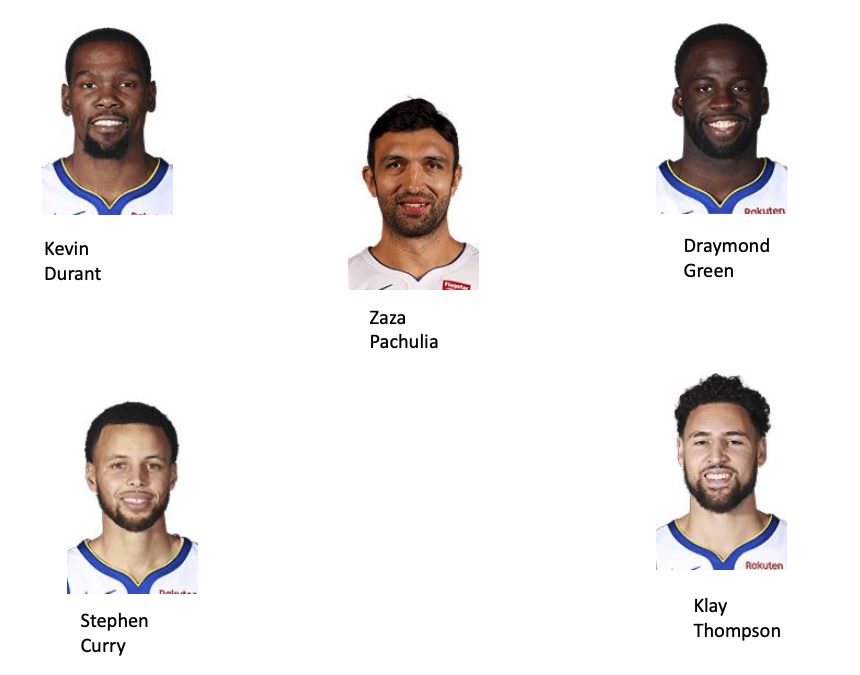
\includegraphics[width=0.9\linewidth,height=0.8\textheight]{./images/nba_squad}
\ecenter
\end{frame}

\begin{frame}[fragile]{NBA: passing network}
\protect\hypertarget{nba-passing-network-30}{}
Create a new network with the given lineup

\begin{Shaded}
\begin{Highlighting}[]
\NormalTok{lineup }\OtherTok{\textless{}{-}} \FunctionTok{c}\NormalTok{(}\StringTok{"Kevin Durant"}\NormalTok{, }\StringTok{"Zaza Pachulia"}\NormalTok{, }
            \StringTok{"Draymond Green"}\NormalTok{, }\StringTok{"Stephen Curry"}\NormalTok{,}
            \StringTok{"Klay Thompson"}\NormalTok{)}
\NormalTok{n\_pass2 }\OtherTok{\textless{}{-}} \FunctionTok{get.inducedSubgraph}\NormalTok{(n\_pass1, }
            \AttributeTok{v=}\FunctionTok{which}\NormalTok{(n\_pass1 }\SpecialCharTok{\%v\%} \StringTok{"vertex.names"}  \SpecialCharTok{\%in\%}\NormalTok{ lineup))}
\end{Highlighting}
\end{Shaded}
\end{frame}

\begin{frame}[fragile]{NBA: passing network}
\protect\hypertarget{nba-passing-network-31}{}
Plot with two additional arguments \tiny

\begin{Shaded}
\begin{Highlighting}[]
\FunctionTok{plot}\NormalTok{(n\_pass2, }\AttributeTok{displaylabels=}\NormalTok{T, }
      \AttributeTok{usecurve=}\NormalTok{T, }\AttributeTok{edge.curve=}\FloatTok{0.025}\NormalTok{)}
\end{Highlighting}
\end{Shaded}

\begin{center}\includegraphics[height=0.65\textheight]{network_analysis_files/figure-beamer/unnamed-chunk-104-1} \end{center}
\end{frame}

\begin{frame}[fragile]{NBA: passing network}
\protect\hypertarget{nba-passing-network-32}{}
\tiny

\begin{Shaded}
\begin{Highlighting}[]
\NormalTok{coords }\OtherTok{\textless{}{-}} \FunctionTok{plot}\NormalTok{(n\_pass2, }\AttributeTok{displaylabels=}\NormalTok{T, }
      \AttributeTok{suppress.axes =}\NormalTok{ F)}
\end{Highlighting}
\end{Shaded}

\begin{center}\includegraphics[height=0.75\textheight]{network_analysis_files/figure-beamer/unnamed-chunk-105-1} \end{center}
\end{frame}

\begin{frame}[fragile]{NBA: passing network}
\protect\hypertarget{nba-passing-network-33}{}
We can try to change the coordinates

\begin{Shaded}
\begin{Highlighting}[]
\NormalTok{coords}
\end{Highlighting}
\end{Shaded}

\begin{verbatim}
##             cx        cy
## [1,] -2.910352 -2.694570
## [2,] -4.012951 -2.751592
## [3,] -3.520333 -1.062279
## [4,] -4.404068 -1.749408
## [5,] -2.625655 -1.662598
\end{verbatim}

\begin{Shaded}
\begin{Highlighting}[]
\NormalTok{n\_pass2 }\SpecialCharTok{\%v\%} \StringTok{"vertex.names"}
\end{Highlighting}
\end{Shaded}

\begin{verbatim}
## [1] "Draymond Green" "Klay Thompson"  "Stephen Curry"  "Kevin Durant"  
## [5] "Zaza Pachulia"
\end{verbatim}
\end{frame}

\begin{frame}[fragile]{NBA: passing network}
\protect\hypertarget{nba-passing-network-34}{}
\begin{Shaded}
\begin{Highlighting}[]
\CommentTok{\# "Draymond Green"}
\NormalTok{coords[}\DecValTok{1}\NormalTok{,] }\OtherTok{\textless{}{-}} \FunctionTok{c}\NormalTok{(}\SpecialCharTok{{-}}\DecValTok{2}\NormalTok{, }\SpecialCharTok{{-}}\DecValTok{3}\NormalTok{)}
\CommentTok{\# "Klay Thompson"}
\NormalTok{coords[}\DecValTok{2}\NormalTok{,] }\OtherTok{\textless{}{-}} \FunctionTok{c}\NormalTok{(}\SpecialCharTok{{-}}\DecValTok{2}\NormalTok{, }\SpecialCharTok{{-}}\FloatTok{4.2}\NormalTok{)}
\CommentTok{\# "Stephen Curry"}
\NormalTok{coords[}\DecValTok{3}\NormalTok{,] }\OtherTok{\textless{}{-}} \FunctionTok{c}\NormalTok{(}\SpecialCharTok{{-}}\FloatTok{3.5}\NormalTok{, }\SpecialCharTok{{-}}\FloatTok{4.5}\NormalTok{)}
\CommentTok{\# "Kevin Durant"}
\NormalTok{coords[}\DecValTok{4}\NormalTok{,] }\OtherTok{\textless{}{-}} \FunctionTok{c}\NormalTok{(}\SpecialCharTok{{-}}\FloatTok{3.6}\NormalTok{, }\SpecialCharTok{{-}}\DecValTok{3}\NormalTok{)}
\CommentTok{\# "Zaza Pachulia"}
\NormalTok{coords[}\DecValTok{5}\NormalTok{,] }\OtherTok{\textless{}{-}} \FunctionTok{c}\NormalTok{(}\SpecialCharTok{{-}}\FloatTok{2.7}\NormalTok{, }\SpecialCharTok{{-}}\FloatTok{3.2}\NormalTok{)}
\end{Highlighting}
\end{Shaded}
\end{frame}

\begin{frame}[fragile]{NBA: passing network}
\protect\hypertarget{nba-passing-network-35}{}
\tiny

\begin{Shaded}
\begin{Highlighting}[]
\FunctionTok{plot}\NormalTok{(n\_pass2, }\AttributeTok{displaylabels=}\NormalTok{T, }\AttributeTok{coord =}\NormalTok{ coords,}
     \AttributeTok{usecurve=}\NormalTok{T, }\AttributeTok{edge.curve=}\FloatTok{0.015}\NormalTok{)}
\end{Highlighting}
\end{Shaded}

\begin{center}\includegraphics[height=0.75\textheight]{network_analysis_files/figure-beamer/unnamed-chunk-108-1} \end{center}
\end{frame}

\begin{frame}[fragile]{NBA: passing network}
\protect\hypertarget{nba-passing-network-36}{}
Number of passes as edge attribute

\tiny

\begin{Shaded}
\begin{Highlighting}[]
\NormalTok{z }\OtherTok{\textless{}{-}} \DecValTok{10}\SpecialCharTok{*}\NormalTok{(x }\SpecialCharTok{{-}} \FunctionTok{min}\NormalTok{(x))}\SpecialCharTok{/}\NormalTok{(}\FunctionTok{max}\NormalTok{(x)}\SpecialCharTok{{-}}\FunctionTok{min}\NormalTok{(x))}
\FunctionTok{plot}\NormalTok{(n\_pass2, }\AttributeTok{displaylabels=}\NormalTok{T, }\AttributeTok{coord =}\NormalTok{ coords,}
     \AttributeTok{usecurve=}\NormalTok{T, }\AttributeTok{edge.curve=}\FloatTok{0.015}\NormalTok{, }
     \AttributeTok{edge.lwd =}\NormalTok{ z)}
\end{Highlighting}
\end{Shaded}

\begin{center}\includegraphics[height=0.65\textheight]{network_analysis_files/figure-beamer/unnamed-chunk-109-1} \end{center}
\end{frame}

\begin{frame}[fragile]{NBA: passing network}
\protect\hypertarget{nba-passing-network-37}{}
Field goal percentage in each edge

\tiny

\begin{Shaded}
\begin{Highlighting}[]
\FunctionTok{plot}\NormalTok{(n\_pass2, }\AttributeTok{displaylabels=}\NormalTok{T, }\AttributeTok{coord =}\NormalTok{ coords,}
     \AttributeTok{usecurve=}\NormalTok{T, }\AttributeTok{edge.curve=}\FloatTok{0.015}\NormalTok{, }
     \AttributeTok{edge.label =}\NormalTok{ n\_pass2 }\SpecialCharTok{\%e\%} \StringTok{"FGP"}\NormalTok{)}
\end{Highlighting}
\end{Shaded}

\begin{center}\includegraphics[height=0.65\textheight]{network_analysis_files/figure-beamer/unnamed-chunk-110-1} \end{center}
\end{frame}

\begin{frame}[fragile]{NBA: passing network}
\protect\hypertarget{nba-passing-network-38}{}
\tiny

\begin{Shaded}
\begin{Highlighting}[]
\NormalTok{i\_pass2 }\OtherTok{\textless{}{-}}\NormalTok{ intergraph}\SpecialCharTok{::}\FunctionTok{asIgraph}\NormalTok{(n\_pass2)}
\FunctionTok{plot}\NormalTok{(i\_pass2, }\AttributeTok{vertex.label =} \FunctionTok{V}\NormalTok{(i\_pass2)}\SpecialCharTok{$}\NormalTok{vertex.names)}
\end{Highlighting}
\end{Shaded}

\begin{center}\includegraphics[height=0.75\textheight]{network_analysis_files/figure-beamer/unnamed-chunk-111-1} \end{center}
\end{frame}

\begin{frame}[fragile]{NBA: passing network}
\protect\hypertarget{nba-passing-network-39}{}
\tiny

\begin{Shaded}
\begin{Highlighting}[]
\FunctionTok{plot}\NormalTok{(i\_pass2, }\AttributeTok{vertex.label =} \FunctionTok{V}\NormalTok{(i\_pass2)}\SpecialCharTok{$}\NormalTok{vertex.names,}
     \AttributeTok{layout=}\NormalTok{coords)}
\end{Highlighting}
\end{Shaded}

\begin{center}\includegraphics[height=0.75\textheight]{network_analysis_files/figure-beamer/unnamed-chunk-112-1} \end{center}
\end{frame}

\begin{frame}[fragile]{NBA: passing network}
\protect\hypertarget{nba-passing-network-40}{}
\tiny

\begin{Shaded}
\begin{Highlighting}[]
\NormalTok{x }\OtherTok{\textless{}{-}} \FunctionTok{E}\NormalTok{(i\_pass2)}\SpecialCharTok{$}\NormalTok{passes}
\NormalTok{z }\OtherTok{\textless{}{-}} \DecValTok{10}\SpecialCharTok{*}\NormalTok{(x }\SpecialCharTok{{-}} \FunctionTok{min}\NormalTok{(x))}\SpecialCharTok{/}\NormalTok{(}\FunctionTok{max}\NormalTok{(x)}\SpecialCharTok{{-}}\FunctionTok{min}\NormalTok{(x))}

\FunctionTok{plot}\NormalTok{(i\_pass2, }\AttributeTok{vertex.label =} \FunctionTok{V}\NormalTok{(i\_pass2)}\SpecialCharTok{$}\NormalTok{vertex.names,}
     \AttributeTok{layout=}\NormalTok{coords, }\AttributeTok{edge.width =}\NormalTok{ z, }\AttributeTok{edge.curved=}\FloatTok{0.2}\NormalTok{)}
\end{Highlighting}
\end{Shaded}

\begin{center}\includegraphics[height=0.75\textheight]{network_analysis_files/figure-beamer/unnamed-chunk-113-1} \end{center}
\end{frame}

\begin{frame}{Passing in football}
\protect\hypertarget{passing-in-football}{}
\begin{block}{Passing in football}
\protect\hypertarget{passing-in-football-1}{}
\end{block}
\end{frame}

\begin{frame}{Passing in football}
\protect\hypertarget{passing-in-football-2}{}
\begin{col}{0.55\textwidth}
World cup final Germany 1-0 Argentina

\end{col}

\begin{col}{0.05\textwidth}
~

\end{col}

\begin{col}{0.4\textwidth}
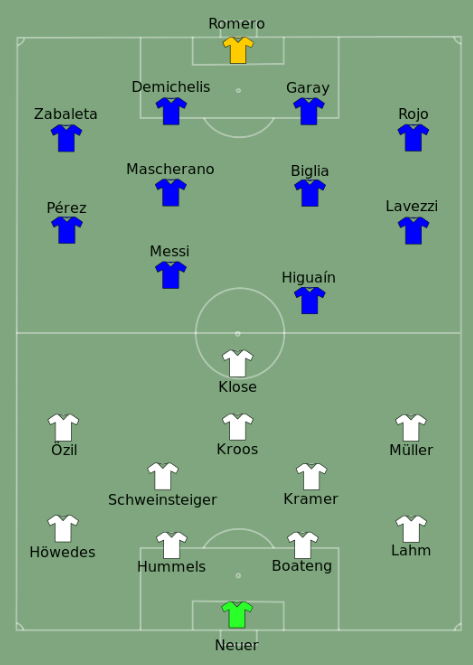
\includegraphics[width=0.9\linewidth,height=0.9\textheight]{./images/wc_14}

\end{col}

::::::
\end{frame}

\begin{frame}[fragile]{Passing in football}
\protect\hypertarget{passing-in-football-3}{}
\begin{Shaded}
\begin{Highlighting}[]
\FunctionTok{data}\NormalTok{(}\StringTok{"wc\_14\_final"}\NormalTok{)}
\FunctionTok{names}\NormalTok{(wc\_14\_final)}
\end{Highlighting}
\end{Shaded}

\begin{verbatim}
## [1] "argentina_team"    "argentina_passing" "germany_team"     
## [4] "germany_passing"
\end{verbatim}

The passing network is given in the form of adjacency matrix

\begin{Shaded}
\begin{Highlighting}[]
\FunctionTok{dim}\NormalTok{(wc\_14\_final}\SpecialCharTok{$}\NormalTok{argentina\_passing)}
\end{Highlighting}
\end{Shaded}

\begin{verbatim}
## [1] 14 14
\end{verbatim}
\end{frame}

\begin{frame}[fragile]{Passing in football}
\protect\hypertarget{passing-in-football-4}{}
\begin{Shaded}
\begin{Highlighting}[]
\FunctionTok{head}\NormalTok{(wc\_14\_final}\SpecialCharTok{$}\NormalTok{argentina\_team)}
\end{Highlighting}
\end{Shaded}

\begin{verbatim}
##       Player_name Shirt_number Position Played_minutes Long_completed
## 1   Sergio ROMERO            1       GK        129'09"              8
## 2  Ezequiel GARAY            2       DF        129'09"              8
## 3  Pablo ZABALETA            4       DF        129'09"              3
## 4    Lucas BIGLIA            6       MF        129'09"              7
## 5      Enzo PEREZ            8       MF         87'59"              1
## 6 Gonzalo HIGUAIN            9       FW         79'23"              0
##   Long_attempted Medium_completed Medium_attempted Short_completed
## 1             30               11               11               1
## 2             10               30               35               5
## 3              8               33               39              11
## 4              9               30               38               6
## 5              1               16               20               9
## 6              0                7               10               7
##   Short_attempted Pass_completed Pass_attempted
## 1               1             20             42
## 2               7             43             52
## 3              17             47             64
## 4              11             43             58
## 5              14             26             35
## 6               8             14             18
\end{verbatim}
\end{frame}

\begin{frame}[fragile]{Passing in football}
\protect\hypertarget{passing-in-football-5}{}
\begin{Shaded}
\begin{Highlighting}[]
\NormalTok{i\_arg }\OtherTok{\textless{}{-}}\NormalTok{ igraph}\SpecialCharTok{::}\FunctionTok{graph.adjacency}\NormalTok{(}\FunctionTok{as.matrix}\NormalTok{(wc\_14\_final}\SpecialCharTok{$}\NormalTok{argentina\_passing),}
                               \AttributeTok{mode=}\StringTok{"directed"}\NormalTok{,}\AttributeTok{weighted=}\ConstantTok{TRUE}\NormalTok{,}\AttributeTok{diag=}\ConstantTok{FALSE}\NormalTok{)}
\NormalTok{net\_arg }\OtherTok{\textless{}{-}}\NormalTok{ intergraph}\SpecialCharTok{::}\FunctionTok{asNetwork}\NormalTok{(i\_arg)}
\end{Highlighting}
\end{Shaded}

\begin{Shaded}
\begin{Highlighting}[]
\FunctionTok{list.edge.attributes}\NormalTok{(net\_arg)}
\end{Highlighting}
\end{Shaded}

\begin{verbatim}
## [1] "na"     "weight"
\end{verbatim}

\begin{Shaded}
\begin{Highlighting}[]
\FunctionTok{list.vertex.attributes}\NormalTok{(net\_arg)}
\end{Highlighting}
\end{Shaded}

\begin{verbatim}
## [1] "na"           "vertex.names"
\end{verbatim}
\end{frame}

\begin{frame}[fragile]{Passing in football}
\protect\hypertarget{passing-in-football-6}{}
Adding vertex attributes

Player positions

\begin{Shaded}
\begin{Highlighting}[]
\NormalTok{network}\SpecialCharTok{::}\FunctionTok{set.vertex.attribute}\NormalTok{(net\_arg, }\StringTok{"player.name"}\NormalTok{,}
\NormalTok{          wc\_14\_final}\SpecialCharTok{$}\NormalTok{argentina\_team}\SpecialCharTok{$}\NormalTok{Player\_name)}
\FunctionTok{get.vertex.attribute}\NormalTok{(net\_arg, }\StringTok{"player.name"}\NormalTok{)}
\end{Highlighting}
\end{Shaded}

\begin{verbatim}
##  [1] "Sergio ROMERO"     "Ezequiel GARAY"    "Pablo ZABALETA"   
##  [4] "Lucas BIGLIA"      "Enzo PEREZ"        "Gonzalo HIGUAIN"  
##  [7] "Lionel MESSI"      "Javier MASCHERANO" "Martin DEMICHELIS"
## [10] "Marcos ROJO"       "Ezequiel LAVEZZI"  "Fernando GAGO"    
## [13] "Rodrigo PALACIO"   "Sergio AGUERO"
\end{verbatim}

\begin{Shaded}
\begin{Highlighting}[]
\NormalTok{network}\SpecialCharTok{::}\FunctionTok{set.vertex.attribute}\NormalTok{(net\_arg, }\StringTok{"player.position"}\NormalTok{,}
        \FunctionTok{as.character}\NormalTok{(wc\_14\_final}\SpecialCharTok{$}\NormalTok{argentina\_team}\SpecialCharTok{$}\NormalTok{Position))}
\FunctionTok{get.vertex.attribute}\NormalTok{(net\_arg, }\StringTok{"player.position"}\NormalTok{)}
\end{Highlighting}
\end{Shaded}

\begin{verbatim}
##  [1] "GK" "DF" "DF" "MF" "MF" "FW" "FW" "MF" "DF" "DF" "FW" "MF" "FW" "FW"
\end{verbatim}
\end{frame}

\begin{frame}[fragile]{Passing in football}
\protect\hypertarget{passing-in-football-7}{}
Number of completed passes and completion \%

\begin{Shaded}
\begin{Highlighting}[]
\NormalTok{network}\SpecialCharTok{::}\FunctionTok{set.vertex.attribute}\NormalTok{(net\_arg, }\StringTok{"passes.completed"}\NormalTok{,}
\NormalTok{                wc\_14\_final}\SpecialCharTok{$}\NormalTok{argentina\_team}\SpecialCharTok{$}\NormalTok{Pass\_completed)}
\end{Highlighting}
\end{Shaded}

\begin{Shaded}
\begin{Highlighting}[]
\NormalTok{wc\_14\_final}\SpecialCharTok{$}\NormalTok{argentina\_team}\SpecialCharTok{$}\NormalTok{Completion }\OtherTok{\textless{}{-}}\NormalTok{ wc\_14\_final}\SpecialCharTok{$}\NormalTok{argentina\_team}\SpecialCharTok{$}\NormalTok{Pass\_completed}\SpecialCharTok{/}
\NormalTok{  wc\_14\_final}\SpecialCharTok{$}\NormalTok{argentina\_team}\SpecialCharTok{$}\NormalTok{Pass\_attempted}
\end{Highlighting}
\end{Shaded}

\begin{Shaded}
\begin{Highlighting}[]
\NormalTok{network}\SpecialCharTok{::}\FunctionTok{set.vertex.attribute}\NormalTok{(net\_arg, }\StringTok{"completion"}\NormalTok{,}
\NormalTok{                wc\_14\_final}\SpecialCharTok{$}\NormalTok{argentina\_team}\SpecialCharTok{$}\NormalTok{Completion)}
\FunctionTok{get.vertex.attribute}\NormalTok{(net\_arg, }\StringTok{"completion"}\NormalTok{)}
\end{Highlighting}
\end{Shaded}

\begin{verbatim}
##  [1] 0.4761905 0.8269231 0.7343750 0.7413793 0.7428571 0.7777778 0.6086957
##  [8] 0.7837838 0.8363636 0.6885246 0.3684211 0.8333333 0.5000000 0.6071429
\end{verbatim}
\end{frame}

\begin{frame}[fragile]{Passing in football}
\protect\hypertarget{passing-in-football-8}{}
Create a subgraph with starting 11 only

\begin{Shaded}
\begin{Highlighting}[]
\NormalTok{net\_st }\OtherTok{\textless{}{-}} \FunctionTok{get.inducedSubgraph}\NormalTok{(net\_arg, }\AttributeTok{v=}\DecValTok{1}\SpecialCharTok{:}\DecValTok{11}\NormalTok{)}
\FunctionTok{get.vertex.attribute}\NormalTok{(net\_st, }\StringTok{"player.name"}\NormalTok{)}
\end{Highlighting}
\end{Shaded}

\begin{verbatim}
##  [1] "Sergio ROMERO"     "Ezequiel GARAY"    "Pablo ZABALETA"   
##  [4] "Lucas BIGLIA"      "Enzo PEREZ"        "Gonzalo HIGUAIN"  
##  [7] "Lionel MESSI"      "Javier MASCHERANO" "Martin DEMICHELIS"
## [10] "Marcos ROJO"       "Ezequiel LAVEZZI"
\end{verbatim}
\end{frame}

\begin{frame}[fragile]{Passing in football}
\protect\hypertarget{passing-in-football-9}{}
\begin{itemize}
\tightlist
\item
  Random layout
\item
  Save the coordinates
\end{itemize}

\tiny

\begin{Shaded}
\begin{Highlighting}[]
\FunctionTok{set.seed}\NormalTok{(}\DecValTok{1}\NormalTok{)}
\NormalTok{coords }\OtherTok{\textless{}{-}} \FunctionTok{plot}\NormalTok{(net\_st, }\AttributeTok{suppress.axes=}\NormalTok{F)}
\end{Highlighting}
\end{Shaded}

\includegraphics[height=0.8\textheight]{network_analysis_files/figure-beamer/unnamed-chunk-125-1}
\end{frame}

\begin{frame}{Passing in football}
\protect\hypertarget{passing-in-football-10}{}
\begin{col}{0.55\textwidth}
Change the coordinates to get approximate positions of the players on
the field

\end{col}

\begin{col}{0.05\textwidth}
~

\end{col}

\begin{col}{0.4\textwidth}
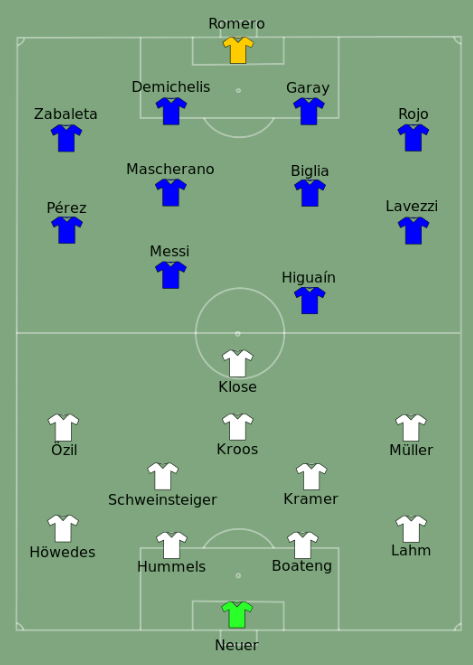
\includegraphics[width=0.9\linewidth,height=0.9\textheight]{./images/wc_14}

\end{col}

::::::
\end{frame}

\begin{frame}[fragile]{Passing in football}
\protect\hypertarget{passing-in-football-11}{}
\begin{Shaded}
\begin{Highlighting}[]
\CommentTok{\# The goalkeeper}
\NormalTok{coords[}\DecValTok{1}\NormalTok{,] }\OtherTok{\textless{}{-}} \FunctionTok{c}\NormalTok{(}\DecValTok{7}\NormalTok{,}\DecValTok{2}\NormalTok{)}
\CommentTok{\# Garay}
\NormalTok{coords[}\DecValTok{2}\NormalTok{,] }\OtherTok{\textless{}{-}} \FunctionTok{c}\NormalTok{(}\DecValTok{8}\NormalTok{, }\FloatTok{3.5}\NormalTok{)}
\CommentTok{\# Demichelis}
\NormalTok{coords[}\DecValTok{9}\NormalTok{,] }\OtherTok{\textless{}{-}} \FunctionTok{c}\NormalTok{(}\DecValTok{8}\NormalTok{, }\FloatTok{0.5}\NormalTok{)}
\CommentTok{\# Zabaleta}
\NormalTok{coords[}\DecValTok{3}\NormalTok{,] }\OtherTok{\textless{}{-}} \FunctionTok{c}\NormalTok{(}\DecValTok{9}\NormalTok{,}\FloatTok{4.5}\NormalTok{)}
\CommentTok{\# Rojo}
\NormalTok{coords[}\DecValTok{10}\NormalTok{,] }\OtherTok{\textless{}{-}} \FunctionTok{c}\NormalTok{(}\DecValTok{9}\NormalTok{, }\SpecialCharTok{{-}}\DecValTok{1}\NormalTok{)}
\CommentTok{\# Biglia}
\NormalTok{coords[}\DecValTok{4}\NormalTok{,] }\OtherTok{\textless{}{-}} \FunctionTok{c}\NormalTok{(}\FloatTok{10.5}\NormalTok{, }\FloatTok{3.5}\NormalTok{)}
\CommentTok{\# Mascherano}
\NormalTok{coords[}\DecValTok{8}\NormalTok{,] }\OtherTok{\textless{}{-}} \FunctionTok{c}\NormalTok{(}\FloatTok{10.5}\NormalTok{, }\FloatTok{0.5}\NormalTok{)}
\CommentTok{\# Perez}
\NormalTok{coords[}\DecValTok{5}\NormalTok{,] }\OtherTok{\textless{}{-}} \FunctionTok{c}\NormalTok{(}\FloatTok{11.5}\NormalTok{, }\SpecialCharTok{{-}}\DecValTok{1}\NormalTok{)}
\CommentTok{\# Lavezzi}
\NormalTok{coords[}\DecValTok{11}\NormalTok{,] }\OtherTok{\textless{}{-}} \FunctionTok{c}\NormalTok{(}\FloatTok{11.5}\NormalTok{,}\FloatTok{4.5}\NormalTok{)}
\CommentTok{\#Messi}
\NormalTok{coords[}\DecValTok{7}\NormalTok{,] }\OtherTok{\textless{}{-}} \FunctionTok{c}\NormalTok{(}\FloatTok{13.5}\NormalTok{, }\FloatTok{0.5}\NormalTok{)}
\CommentTok{\# Higuain}
\NormalTok{coords[}\DecValTok{6}\NormalTok{,] }\OtherTok{\textless{}{-}} \FunctionTok{c}\NormalTok{(}\FloatTok{14.5}\NormalTok{, }\FloatTok{3.5}\NormalTok{)}
\end{Highlighting}
\end{Shaded}
\end{frame}

\begin{frame}[fragile]{Passing in football}
\protect\hypertarget{passing-in-football-12}{}
\tiny

\begin{Shaded}
\begin{Highlighting}[]
\FunctionTok{plot}\NormalTok{(net\_st, }\AttributeTok{coord=}\NormalTok{coords, }\AttributeTok{suppress.axes=}\NormalTok{F, }
     \AttributeTok{label =}\NormalTok{ net\_st }\SpecialCharTok{\%v\%} \StringTok{"player.name"}\NormalTok{)}
\end{Highlighting}
\end{Shaded}

\includegraphics[height=0.8\textheight]{network_analysis_files/figure-beamer/unnamed-chunk-128-1}
\end{frame}

\begin{frame}[fragile]{Passing in football}
\protect\hypertarget{passing-in-football-13}{}
Passing density \tiny

\begin{Shaded}
\begin{Highlighting}[]
\FunctionTok{plot}\NormalTok{(net\_st, }\AttributeTok{vertex.col=}\StringTok{"player.position"}\NormalTok{, }\AttributeTok{edge.lwd=}\StringTok{"weight"}\NormalTok{,}
     \AttributeTok{coord=}\NormalTok{coords)}
\end{Highlighting}
\end{Shaded}

\includegraphics[height=0.8\textheight]{network_analysis_files/figure-beamer/unnamed-chunk-129-1}
\end{frame}

\begin{frame}[fragile]{Passing in football}
\protect\hypertarget{passing-in-football-14}{}
Completion rate \tiny

\begin{Shaded}
\begin{Highlighting}[]
\FunctionTok{plot}\NormalTok{(net\_st, }\AttributeTok{vertex.col=}\StringTok{"player.position"}\NormalTok{,}
     \AttributeTok{coord=}\NormalTok{coords, }\AttributeTok{vertex.cex =} \DecValTok{2}\SpecialCharTok{*}\NormalTok{(net\_st }\SpecialCharTok{\%v\%} \StringTok{"completion"}\NormalTok{),}
     \AttributeTok{label =}\NormalTok{ net\_st }\SpecialCharTok{\%v\%} \StringTok{"player.name"}\NormalTok{)}
\end{Highlighting}
\end{Shaded}

\includegraphics{network_analysis_files/figure-beamer/unnamed-chunk-130-1.pdf}
\end{frame}

\begin{frame}[fragile]{Passing in football}
\protect\hypertarget{passing-in-football-15}{}
Last: create a chord diagram

\begin{Shaded}
\begin{Highlighting}[]
\NormalTok{st\_mat }\OtherTok{\textless{}{-}} \FunctionTok{as.matrix}\NormalTok{(net\_st, }\AttributeTok{matrix.type =} \StringTok{"adjacency"}\NormalTok{, }\AttributeTok{attrname =} \StringTok{"weight"}\NormalTok{)}
\FunctionTok{colnames}\NormalTok{(st\_mat) }\OtherTok{\textless{}{-}}\NormalTok{ net\_st }\SpecialCharTok{\%v\%} \StringTok{"player.name"}
\FunctionTok{rownames}\NormalTok{(st\_mat) }\OtherTok{\textless{}{-}} \FunctionTok{colnames}\NormalTok{(st\_mat)}
\end{Highlighting}
\end{Shaded}
\end{frame}

\begin{frame}[fragile]{Passing in football}
\protect\hypertarget{passing-in-football-16}{}
\begin{Shaded}
\begin{Highlighting}[]
\FunctionTok{chordDiagram}\NormalTok{(st\_mat, }\AttributeTok{directional =}\NormalTok{ T)}
\end{Highlighting}
\end{Shaded}

\begin{center}\includegraphics[height=0.8\textheight]{network_analysis_files/figure-beamer/unnamed-chunk-132-1} \end{center}
\end{frame}

\end{document}
